% Options for packages loaded elsewhere
\PassOptionsToPackage{unicode}{hyperref}
\PassOptionsToPackage{hyphens}{url}
\PassOptionsToPackage{dvipsnames,svgnames,x11names}{xcolor}
\documentclass[
  10pt,
]{extarticle}
\usepackage{xcolor}
\usepackage[top=1.5in, bottom=1.5in, left=1.5in, right=1.5in]{geometry}
\usepackage{amsmath,amssymb}
\setcounter{secnumdepth}{5}
\usepackage{iftex}
\ifPDFTeX
  \usepackage[T1]{fontenc}
  \usepackage[utf8]{inputenc}
  \usepackage{textcomp} % provide euro and other symbols
\else % if luatex or xetex
  \usepackage{unicode-math} % this also loads fontspec
  \defaultfontfeatures{Scale=MatchLowercase}
  \defaultfontfeatures[\rmfamily]{Ligatures=TeX,Scale=1}
\fi
\usepackage{lmodern}
\ifPDFTeX\else
  % xetex/luatex font selection
\fi
% Use upquote if available, for straight quotes in verbatim environments
\IfFileExists{upquote.sty}{\usepackage{upquote}}{}
\IfFileExists{microtype.sty}{% use microtype if available
  \usepackage[]{microtype}
  \UseMicrotypeSet[protrusion]{basicmath} % disable protrusion for tt fonts
}{}
\makeatletter
\@ifundefined{KOMAClassName}{% if non-KOMA class
  \IfFileExists{parskip.sty}{%
    \usepackage{parskip}
  }{% else
    \setlength{\parindent}{0pt}
    \setlength{\parskip}{6pt plus 2pt minus 1pt}}
}{% if KOMA class
  \KOMAoptions{parskip=half}}
\makeatother
\usepackage{color}
\usepackage{fancyvrb}
\newcommand{\VerbBar}{|}
\newcommand{\VERB}{\Verb[commandchars=\\\{\}]}
\DefineVerbatimEnvironment{Highlighting}{Verbatim}{commandchars=\\\{\}}
% Add ',fontsize=\small' for more characters per line
\usepackage{framed}
\definecolor{shadecolor}{RGB}{248,248,248}
\newenvironment{Shaded}{\begin{snugshade}}{\end{snugshade}}
\newcommand{\AlertTok}[1]{\textcolor[rgb]{0.94,0.16,0.16}{#1}}
\newcommand{\AnnotationTok}[1]{\textcolor[rgb]{0.56,0.35,0.01}{\textbf{\textit{#1}}}}
\newcommand{\AttributeTok}[1]{\textcolor[rgb]{0.13,0.29,0.53}{#1}}
\newcommand{\BaseNTok}[1]{\textcolor[rgb]{0.00,0.00,0.81}{#1}}
\newcommand{\BuiltInTok}[1]{#1}
\newcommand{\CharTok}[1]{\textcolor[rgb]{0.31,0.60,0.02}{#1}}
\newcommand{\CommentTok}[1]{\textcolor[rgb]{0.56,0.35,0.01}{\textit{#1}}}
\newcommand{\CommentVarTok}[1]{\textcolor[rgb]{0.56,0.35,0.01}{\textbf{\textit{#1}}}}
\newcommand{\ConstantTok}[1]{\textcolor[rgb]{0.56,0.35,0.01}{#1}}
\newcommand{\ControlFlowTok}[1]{\textcolor[rgb]{0.13,0.29,0.53}{\textbf{#1}}}
\newcommand{\DataTypeTok}[1]{\textcolor[rgb]{0.13,0.29,0.53}{#1}}
\newcommand{\DecValTok}[1]{\textcolor[rgb]{0.00,0.00,0.81}{#1}}
\newcommand{\DocumentationTok}[1]{\textcolor[rgb]{0.56,0.35,0.01}{\textbf{\textit{#1}}}}
\newcommand{\ErrorTok}[1]{\textcolor[rgb]{0.64,0.00,0.00}{\textbf{#1}}}
\newcommand{\ExtensionTok}[1]{#1}
\newcommand{\FloatTok}[1]{\textcolor[rgb]{0.00,0.00,0.81}{#1}}
\newcommand{\FunctionTok}[1]{\textcolor[rgb]{0.13,0.29,0.53}{\textbf{#1}}}
\newcommand{\ImportTok}[1]{#1}
\newcommand{\InformationTok}[1]{\textcolor[rgb]{0.56,0.35,0.01}{\textbf{\textit{#1}}}}
\newcommand{\KeywordTok}[1]{\textcolor[rgb]{0.13,0.29,0.53}{\textbf{#1}}}
\newcommand{\NormalTok}[1]{#1}
\newcommand{\OperatorTok}[1]{\textcolor[rgb]{0.81,0.36,0.00}{\textbf{#1}}}
\newcommand{\OtherTok}[1]{\textcolor[rgb]{0.56,0.35,0.01}{#1}}
\newcommand{\PreprocessorTok}[1]{\textcolor[rgb]{0.56,0.35,0.01}{\textit{#1}}}
\newcommand{\RegionMarkerTok}[1]{#1}
\newcommand{\SpecialCharTok}[1]{\textcolor[rgb]{0.81,0.36,0.00}{\textbf{#1}}}
\newcommand{\SpecialStringTok}[1]{\textcolor[rgb]{0.31,0.60,0.02}{#1}}
\newcommand{\StringTok}[1]{\textcolor[rgb]{0.31,0.60,0.02}{#1}}
\newcommand{\VariableTok}[1]{\textcolor[rgb]{0.00,0.00,0.00}{#1}}
\newcommand{\VerbatimStringTok}[1]{\textcolor[rgb]{0.31,0.60,0.02}{#1}}
\newcommand{\WarningTok}[1]{\textcolor[rgb]{0.56,0.35,0.01}{\textbf{\textit{#1}}}}
\usepackage{longtable,booktabs,array}
\usepackage{calc} % for calculating minipage widths
% Correct order of tables after \paragraph or \subparagraph
\usepackage{etoolbox}
\makeatletter
\patchcmd\longtable{\par}{\if@noskipsec\mbox{}\fi\par}{}{}
\makeatother
% Allow footnotes in longtable head/foot
\IfFileExists{footnotehyper.sty}{\usepackage{footnotehyper}}{\usepackage{footnote}}
\makesavenoteenv{longtable}
\usepackage{graphicx}
\makeatletter
\newsavebox\pandoc@box
\newcommand*\pandocbounded[1]{% scales image to fit in text height/width
  \sbox\pandoc@box{#1}%
  \Gscale@div\@tempa{\textheight}{\dimexpr\ht\pandoc@box+\dp\pandoc@box\relax}%
  \Gscale@div\@tempb{\linewidth}{\wd\pandoc@box}%
  \ifdim\@tempb\p@<\@tempa\p@\let\@tempa\@tempb\fi% select the smaller of both
  \ifdim\@tempa\p@<\p@\scalebox{\@tempa}{\usebox\pandoc@box}%
  \else\usebox{\pandoc@box}%
  \fi%
}
% Set default figure placement to htbp
\def\fps@figure{htbp}
\makeatother
\setlength{\emergencystretch}{3em} % prevent overfull lines
\providecommand{\tightlist}{%
  \setlength{\itemsep}{0pt}\setlength{\parskip}{0pt}}
\usepackage{xcolor}
\usepackage{hyperref}
\hypersetup{colorlinks=true, linkcolor=blue, urlcolor=blue, citecolor=blue}
\usepackage{float}
\usepackage{fvextra}
\usepackage{fancyhdr}
\usepackage{lastpage}
\usepackage{soul}
\usepackage{etoolbox}
\usepackage{microtype}
\usepackage{tcolorbox}
\usepackage{enumitem}
\usepackage{fancyvrb}
\usepackage{xspace}
\allowdisplaybreaks
\setcounter{tocdepth}{2}
\setcounter{secnumdepth}{0}
\floatplacement{figure}{H}
\makeatletter
\newcommand{\@subtitle}{}
\newcommand{\subtitle}[1]{\gdef\@subtitle{#1}}
\newcommand{\DocSubtitle}{\@subtitle}
\renewcommand{\maketitle}{
  \thispagestyle{plain}
  \null
  \vfill
  \begin{center}
    {\Large \textsc{\@title} \par}\vskip 0.5em
    {\LARGE \bfseries \@subtitle \par}\vskip 0.75em
    {\large \@author \par}\vskip 0.5em
    {\normalsize \@date \par}
  \end{center}
  \vfill
  \tableofcontents
  \vspace{1em}
  \clearpage
}
\AfterEndEnvironment{Highlighting}{\setcounter{CodeLine}{\numexpr\value{CodeLine}+\FV@CodeLineNo\relax}}
\makeatother
\fancypagestyle{plain}{
  \fancyhf{}
  \renewcommand{\headrulewidth}{0pt}
  \renewcommand{\footrulewidth}{0pt}
}
\pagestyle{fancy}
\fancyhf{}
\fancyfoot[C]{\small\textsc{Page}~\thepage~\textsc{of}~\pageref{LastPage}}
\fancyhead[L]{\textsc{Rento Saijo}}
\fancyhead[R]{\textsc{\DocSubtitle}}
\fancyhead[C]{\textsc{\rightmark}}
\renewcommand{\headrulewidth}{0.5pt}
\renewcommand{\footrulewidth}{0.5pt}
\newcounter{CodeLine}
\newcounter{cell}
\AtBeginEnvironment{Highlighting}{\stepcounter{cell}}
\DefineVerbatimEnvironment{Highlighting}{Verbatim}{
  frame=single,
  rulecolor=\color{black},
  framesep=2mm,
  label=\footnotesize Cell \thecell,
  labelposition=topline,
  commandchars=\\\{\},
  breaklines=true,
  breakanywhere=false,
  breaksymbol={},
  numbers=left,
  numbersep=3pt,
  firstnumber=\numexpr\value{CodeLine}+1\relax,
  fontsize=\small
}
\DefineVerbatimEnvironment{verbatim}{Verbatim}{
  breaklines=true,
  breakanywhere=true,
  numbers=left,
  numbersep=3pt,
  firstnumber=1,
  fontsize=\footnotesize
}
\newtcolorbox{problem}[1][]{
  title={\textsc{#1}}
}
\renewcommand{\contentsname}{Table of Contents}
\newcommand{\E}{\mathrm{E}}
\newcommand{\Var}{\mathrm{Var}}
\newcommand{\R}{\textsf{R}\xspace}
\newcommand{\SD}{\mathrm{SD}}
\newcommand{\SE}{\mathrm{SE}}
\usepackage{bookmark}
\IfFileExists{xurl.sty}{\usepackage{xurl}}{} % add URL line breaks if available
\urlstyle{same}
\hypersetup{
  pdftitle={STA 209: Introduction to Time Series Analysis},
  colorlinks=true,
  linkcolor={blue},
  filecolor={Maroon},
  citecolor={blue},
  urlcolor={blue},
  pdfcreator={LaTeX via pandoc}}

\title{STA 209: Introduction to Time Series Analysis}
\usepackage{etoolbox}
\makeatletter
\providecommand{\subtitle}[1]{% add subtitle to \maketitle
  \apptocmd{\@title}{\par {\large #1 \par}}{}{}
}
\makeatother
\subtitle{Homework 4}
\author{Rento Saijo}
\date{March 30, 2026}

\begin{document}
\maketitle

\section{Disclosure}\label{disclosure}

GPT-5.4 Codex was used to create the \texttt{YAML} portion and some \texttt{LaTeX} code to format the text/equations nicely. Page formatting code was also provided by Derin Gezgin. In the setup chunk, chunk options were set for the document. See the original \texttt{RMD} file \href{https://github.com/RentoSaijo/STA209/blob/main/Homework4.Rmd}{here} for more details. Please ignore Problem 2 for this submission.

\newpage

\section{Problem 1}\label{problem-1}

\begin{problem}[Problem 1]
Consider the datasets \texttt{sales} and \texttt{lead} in package \texttt{astsa}.
\end{problem}

\begin{Shaded}
\begin{Highlighting}[]
\CommentTok{\# Load data.}
\NormalTok{sales }\OtherTok{\textless{}{-}}\NormalTok{ astsa}\SpecialCharTok{::}\NormalTok{sales}
\NormalTok{lead  }\OtherTok{\textless{}{-}}\NormalTok{ astsa}\SpecialCharTok{::}\NormalTok{lead}
\end{Highlighting}
\end{Shaded}

The package help states that both series contain 150 observations and are taken from Box and Jenkins (1970). The \texttt{sales} series is monthly sales data and the \texttt{lead} series is the corresponding leading indicator.

\newpage

\subsection{Problem 1 (a)}\label{problem-1-a}

\begin{problem}[Problem 1 (a)]
Plot and comment on the main features of these two time series datasets.
\end{problem}

\begin{Shaded}
\begin{Highlighting}[]
\CommentTok{\# Plot the two original series in separate panels.}
\NormalTok{op }\OtherTok{\textless{}{-}}\NormalTok{ graphics}\SpecialCharTok{::}\FunctionTok{par}\NormalTok{(}\AttributeTok{no.readonly =} \ConstantTok{TRUE}\NormalTok{)}
\FunctionTok{on.exit}\NormalTok{(graphics}\SpecialCharTok{::}\FunctionTok{par}\NormalTok{(op), }\AttributeTok{add =} \ConstantTok{TRUE}\NormalTok{)}
\NormalTok{graphics}\SpecialCharTok{::}\FunctionTok{par}\NormalTok{(}\AttributeTok{mfrow =} \FunctionTok{c}\NormalTok{(}\DecValTok{2}\NormalTok{, }\DecValTok{1}\NormalTok{))}
\NormalTok{astsa}\SpecialCharTok{::}\FunctionTok{tsplot}\NormalTok{(}
\NormalTok{  sales,}
  \AttributeTok{main =} \StringTok{\textquotesingle{}Monthly Sales\textquotesingle{}}\NormalTok{,}
  \AttributeTok{xlab =} \StringTok{\textquotesingle{}Time (Months)\textquotesingle{}}\NormalTok{,}
  \AttributeTok{ylab =} \StringTok{\textquotesingle{}Sales\textquotesingle{}}\NormalTok{,}
  \AttributeTok{col =} \StringTok{\textquotesingle{}firebrick\textquotesingle{}}\NormalTok{,}
  \AttributeTok{lwd =} \DecValTok{2}
\NormalTok{)}
\NormalTok{astsa}\SpecialCharTok{::}\FunctionTok{tsplot}\NormalTok{(}
\NormalTok{  lead,}
  \AttributeTok{main =} \StringTok{\textquotesingle{}Leading Indicator\textquotesingle{}}\NormalTok{,}
  \AttributeTok{xlab =} \StringTok{\textquotesingle{}Time (Months)\textquotesingle{}}\NormalTok{,}
  \AttributeTok{ylab =} \StringTok{\textquotesingle{}Lead\textquotesingle{}}\NormalTok{,}
  \AttributeTok{col =} \StringTok{\textquotesingle{}navy\textquotesingle{}}\NormalTok{,}
  \AttributeTok{lwd =} \DecValTok{2}
\NormalTok{)}
\end{Highlighting}
\end{Shaded}

\begin{center}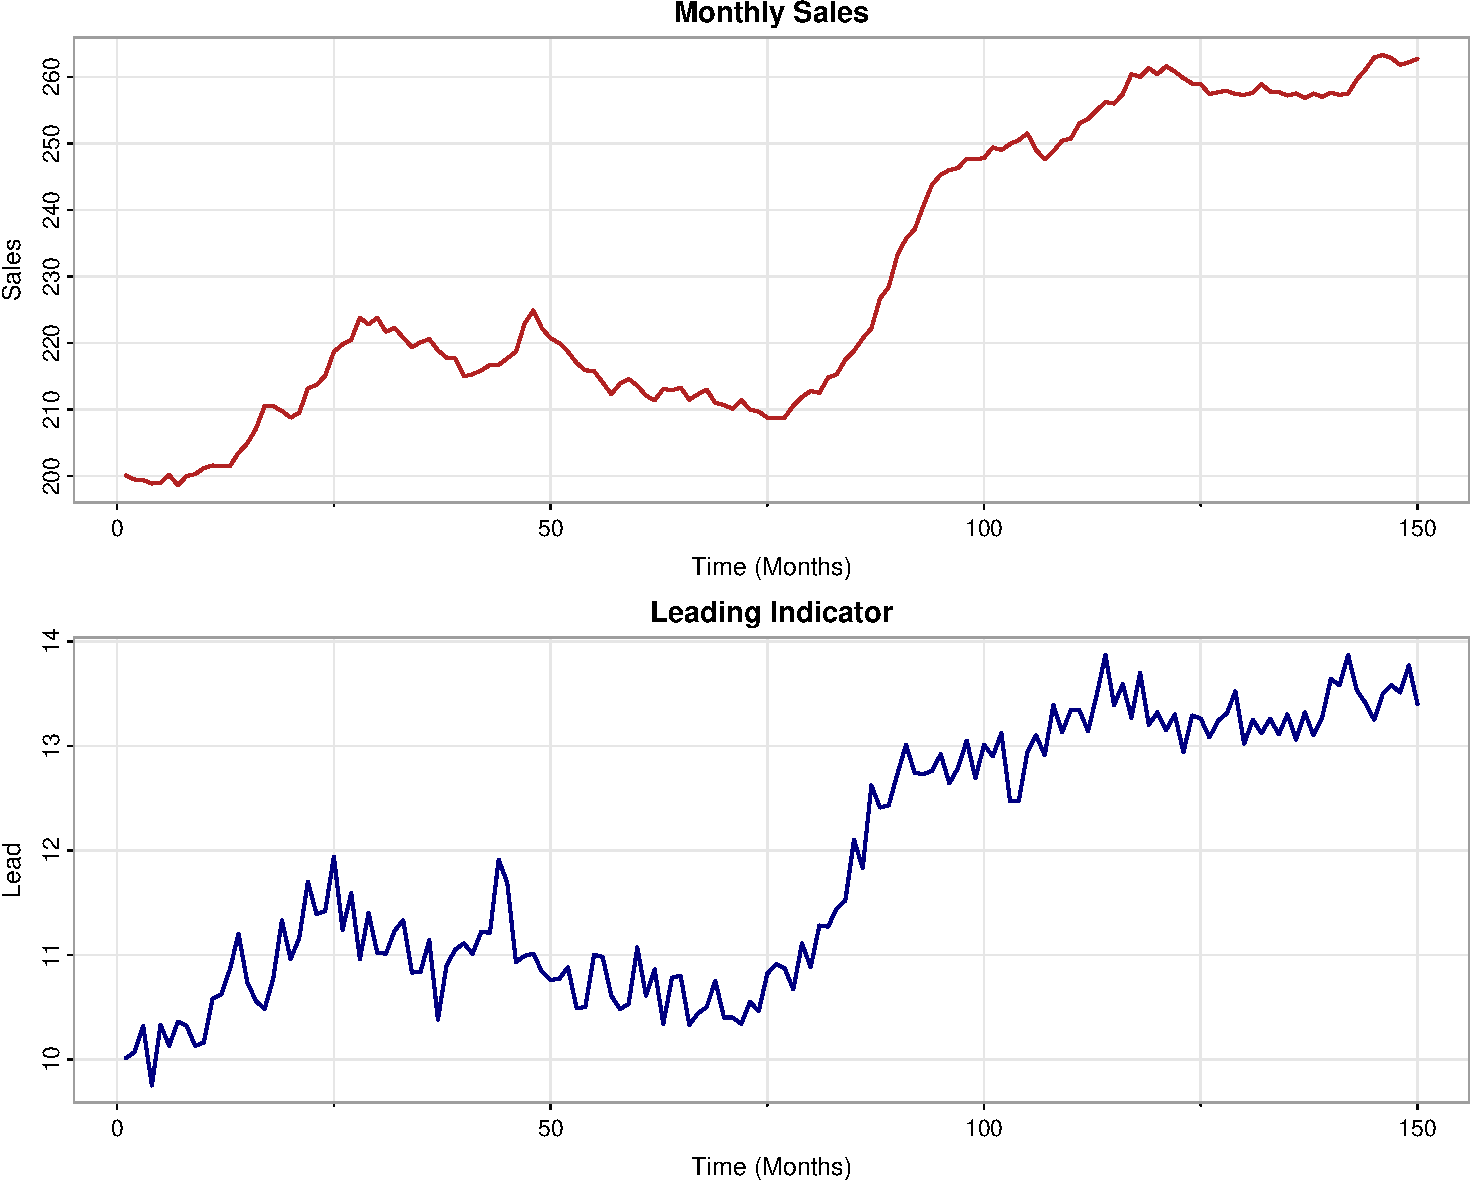
\includegraphics[width=\linewidth]{Homework4_files/figure-latex/unnamed-chunk-3-1} \end{center}

The \texttt{sales} data is a monthly sales time series with 150 observations, so it covers 150 months, or about 12.5 years. The \texttt{lead} data is the monthly leading-indicator time series for the same 150 months. The mean behavior of both series is time-dependent and shows an overall upward trend. For \texttt{sales}, the trend is positive and somewhat nonlinear because the series rises overall, pauses or dips at several points, then increases sharply around the middle-to-late part of the sample before flattening somewhat near the end. For \texttt{lead}, the upward movement is also clear, but it evolves on a smaller scale and with more month-to-month irregular fluctuation than \texttt{sales}. There is no clear repeated seasonal pattern in either plot despite the monthly observation frequency. The variability is moderate in both series, with statistical range \(\max(\texttt{sales})-\min(\texttt{sales}) = 64.7\) and \(\max(\texttt{lead})-\min(\texttt{lead}) = 4.12\). For both, the spread appears fairly stable over time, so there is no strong visual evidence of fanning in or out. The \texttt{sales} series does not look especially volatile, while \texttt{lead} shows more short-run fluctuation, but still no strong volatility clustering.

\newpage

\subsection{Problem 1 (b)}\label{problem-1-b}

\begin{problem}[Problem 1 (b)]
Compute first ordered differenced series for both \texttt{sales} and \texttt{lead}. Show plots of the differenced time series and discuss their main features.
\end{problem}

\begin{Shaded}
\begin{Highlighting}[]
\CommentTok{\# Build first differences.}
\NormalTok{sales.diff }\OtherTok{\textless{}{-}} \FunctionTok{diff}\NormalTok{(sales)}
\NormalTok{lead.diff  }\OtherTok{\textless{}{-}} \FunctionTok{diff}\NormalTok{(lead)}

\CommentTok{\# Plot the differenced series.}
\NormalTok{op }\OtherTok{\textless{}{-}}\NormalTok{ graphics}\SpecialCharTok{::}\FunctionTok{par}\NormalTok{(}\AttributeTok{no.readonly =} \ConstantTok{TRUE}\NormalTok{)}
\FunctionTok{on.exit}\NormalTok{(graphics}\SpecialCharTok{::}\FunctionTok{par}\NormalTok{(op), }\AttributeTok{add =} \ConstantTok{TRUE}\NormalTok{)}
\NormalTok{graphics}\SpecialCharTok{::}\FunctionTok{par}\NormalTok{(}\AttributeTok{mfrow =} \FunctionTok{c}\NormalTok{(}\DecValTok{2}\NormalTok{, }\DecValTok{1}\NormalTok{))}
\NormalTok{astsa}\SpecialCharTok{::}\FunctionTok{tsplot}\NormalTok{(}
\NormalTok{  sales.diff,}
  \AttributeTok{main =} \StringTok{\textquotesingle{}First Difference of Sales\textquotesingle{}}\NormalTok{,}
  \AttributeTok{xlab =} \StringTok{\textquotesingle{}Time (Months)\textquotesingle{}}\NormalTok{,}
  \AttributeTok{ylab =} \StringTok{\textquotesingle{}Monthly Change in Sales\textquotesingle{}}\NormalTok{,}
  \AttributeTok{col =} \StringTok{\textquotesingle{}firebrick\textquotesingle{}}\NormalTok{,}
  \AttributeTok{lwd =} \DecValTok{2}
\NormalTok{)}
\NormalTok{astsa}\SpecialCharTok{::}\FunctionTok{tsplot}\NormalTok{(}
\NormalTok{  lead.diff,}
  \AttributeTok{main =} \StringTok{\textquotesingle{}First Difference of Leading Indicator\textquotesingle{}}\NormalTok{,}
  \AttributeTok{xlab =} \StringTok{\textquotesingle{}Time (Months)\textquotesingle{}}\NormalTok{,}
  \AttributeTok{ylab =} \StringTok{\textquotesingle{}Monthly Change in Lead\textquotesingle{}}\NormalTok{,}
  \AttributeTok{col =} \StringTok{\textquotesingle{}navy\textquotesingle{}}\NormalTok{,}
  \AttributeTok{lwd =} \DecValTok{2}
\NormalTok{)}
\end{Highlighting}
\end{Shaded}

\begin{center}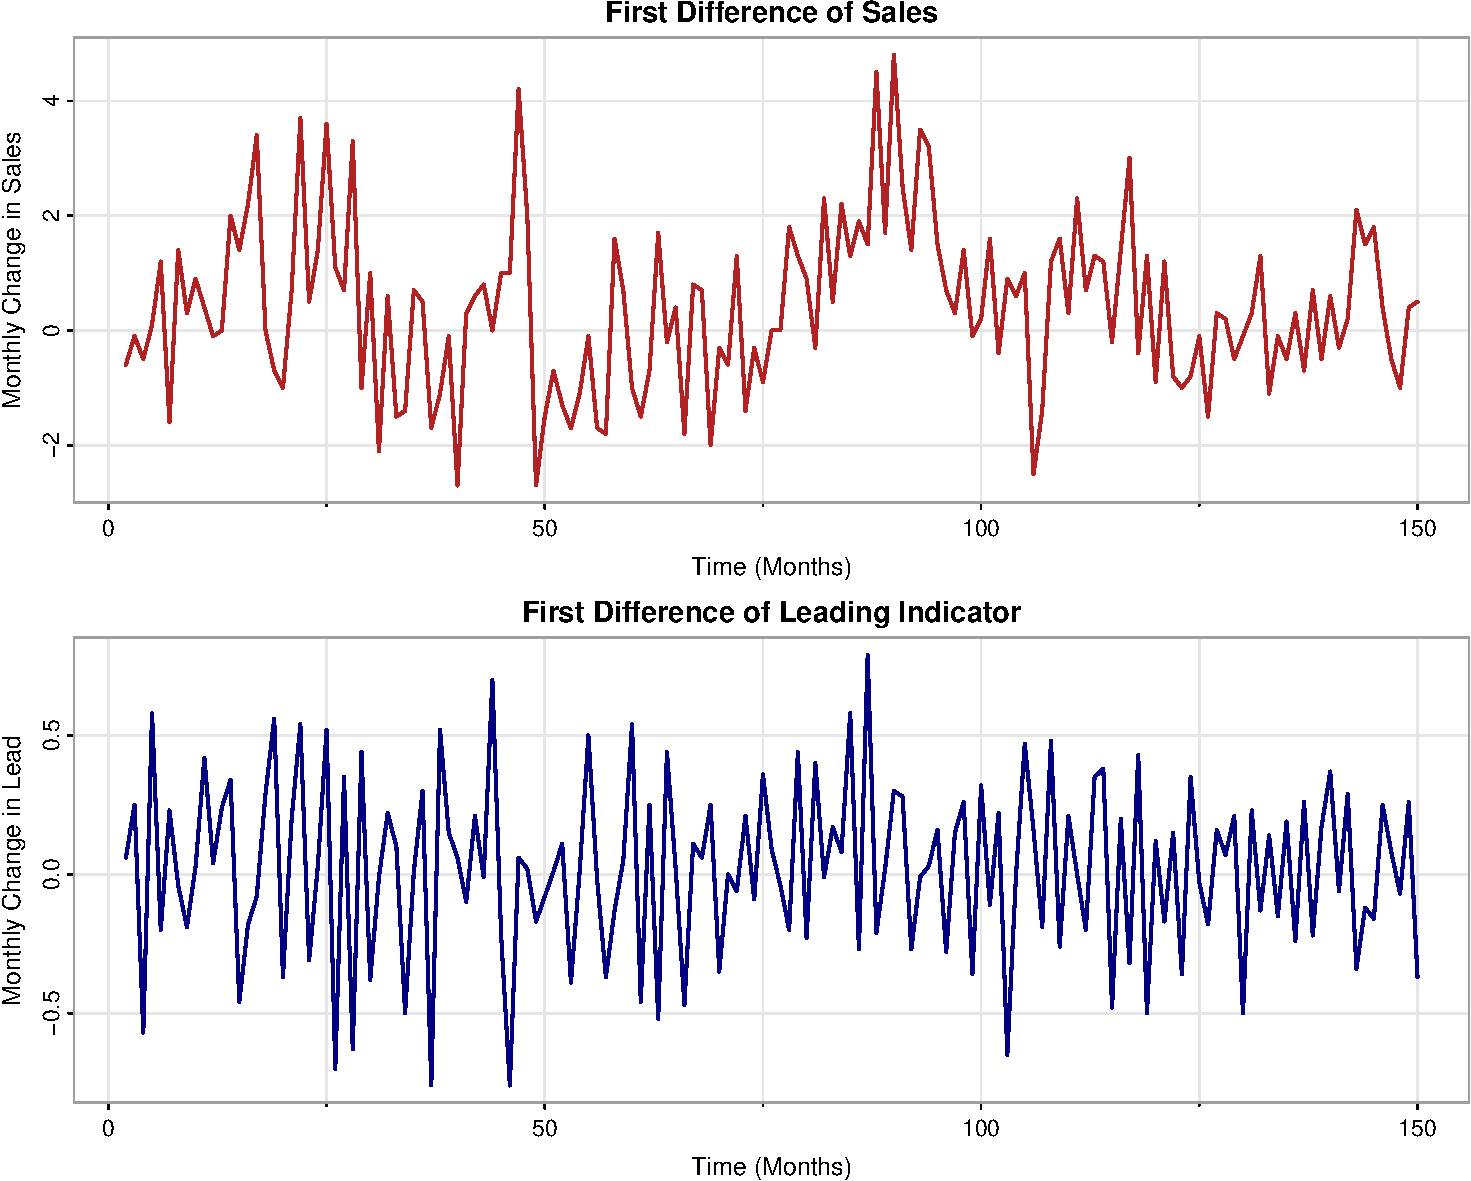
\includegraphics[width=\linewidth]{Homework4_files/figure-latex/unnamed-chunk-4-1} \end{center}

Let \(U_t = \nabla S_t = S_t - S_{t-1}\) and \(V_t = \nabla L_t = L_t - L_{t-1}\). After differencing, both series have 149 observations. The differenced sales series fluctuates around a much more stable level than the original sales series, and the differenced lead series does the same for the leading indicator. In both plots, the major trend has largely been removed, so the mean is much less time-dependent than in part (a). There is still no clear repeated seasonal pattern. The statistical ranges are \(\max(U_t)-\min(U_t) = 7.5\) and \(\max(V_t)-\min(V_t) = 1.55\). The spread looks roughly constant over time, and although there are a few larger jumps, the differenced series are much less variable and much less smooth than the original series. The differenced series also do not look especially volatile; instead, they behave like fairly stable fluctuations around zero with occasional isolated spikes, with \(U_t\) showing the larger jumps and \(V_t\) staying within a narrower band.

\newpage

\subsection{Problem 1 (c)}\label{problem-1-c}

\begin{problem}[Problem 1 (c)]
Plot the CCF of first ordered differenced \texttt{lead} and first ordered differenced \texttt{sales}. Comment on the relation between the two differenced series in specific lead-lag terminology learned in class.
\end{problem}

\begin{Shaded}
\begin{Highlighting}[]
\CommentTok{\# Plot CCF of differenced series.}
\NormalTok{cc.diff }\OtherTok{\textless{}{-}}\NormalTok{ stats}\SpecialCharTok{::}\FunctionTok{ccf}\NormalTok{(}
  \FunctionTok{as.numeric}\NormalTok{(lead.diff),}
  \FunctionTok{as.numeric}\NormalTok{(sales.diff),}
  \AttributeTok{lag.max =} \DecValTok{12}\NormalTok{,}
  \AttributeTok{main =} \StringTok{\textquotesingle{}CCF: Differenced Lead vs Differenced Sales\textquotesingle{}}\NormalTok{,}
  \AttributeTok{ylab =} \StringTok{\textquotesingle{}CCF\textquotesingle{}}
\NormalTok{)}
\end{Highlighting}
\end{Shaded}

\begin{center}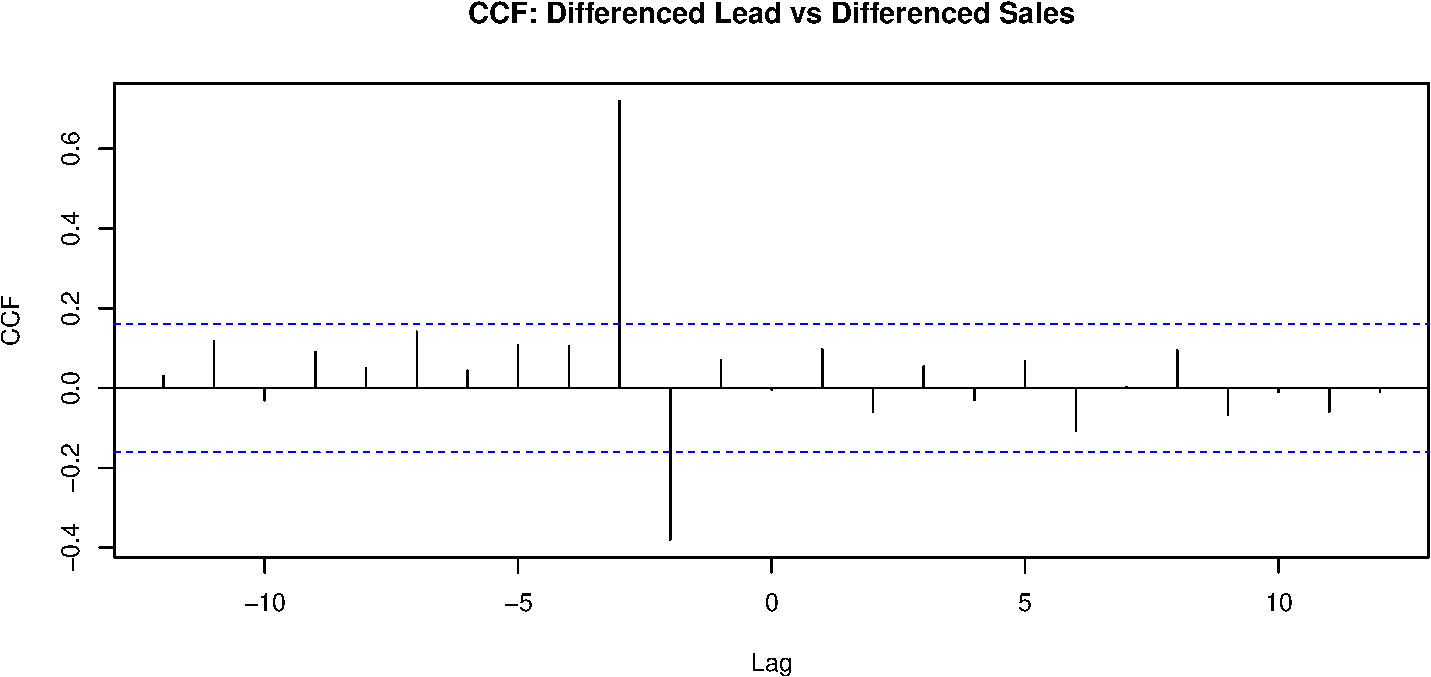
\includegraphics[width=\linewidth]{Homework4_files/figure-latex/unnamed-chunk-5-1} \end{center}

\begin{Shaded}
\begin{Highlighting}[]
\CommentTok{\# Extract dominant lag.}
\NormalTok{cc.max.idx }\OtherTok{\textless{}{-}} \FunctionTok{which.max}\NormalTok{(}\FunctionTok{abs}\NormalTok{(cc.diff}\SpecialCharTok{$}\NormalTok{acf))}
\NormalTok{cc.max.lag }\OtherTok{\textless{}{-}} \FunctionTok{as.numeric}\NormalTok{(cc.diff}\SpecialCharTok{$}\NormalTok{lag[cc.max.idx])}
\NormalTok{cc.max.acf }\OtherTok{\textless{}{-}} \FunctionTok{as.numeric}\NormalTok{(cc.diff}\SpecialCharTok{$}\NormalTok{acf[cc.max.idx])}
\end{Highlighting}
\end{Shaded}

The dominant CCF spike occurs at lag -3 with cross-correlation 0.72. Since the first series passed into \texttt{ccf()} is \texttt{lead.diff}, a negative lag means the differenced leading indicator leads the differenced sales series. Therefore, the CCF indicates that \(V_t\) leads \(U_t\) by 3 months, or equivalently, \(U_t\) lags \(V_t\) by 3 months. The relation is positive at that lag, so increases in the differenced leading indicator tend to be followed by increases in differenced sales about 3 months later.

\newpage

\subsection{Problem 1 (d)}\label{problem-1-d}

\begin{problem}[Problem 1 (d)]
Fit the regression model
\[
\nabla S_t = \beta_0 + \beta_1 \nabla L_{t-3} + X_t,
\]
where \(X_t\) is the residual process after performing regression. Present the fitted model for \(U_t = \nabla S_t\) and discuss how it performed using the details from the summary of this model.
\end{problem}

\begin{Shaded}
\begin{Highlighting}[]
\CommentTok{\# Fit the lag{-}3 regression suggested by the CCF.}
\NormalTok{DiffData }\OtherTok{\textless{}{-}}\NormalTok{ stats}\SpecialCharTok{::}\FunctionTok{ts.intersect}\NormalTok{(}\AttributeTok{U =}\NormalTok{ sales.diff, }\AttributeTok{Lt3 =}\NormalTok{ stats}\SpecialCharTok{::}\FunctionTok{lag}\NormalTok{(lead.diff, }\SpecialCharTok{{-}}\DecValTok{3}\NormalTok{), }\AttributeTok{dframe =} \ConstantTok{TRUE}\NormalTok{)}
\NormalTok{fit }\OtherTok{\textless{}{-}}\NormalTok{ stats}\SpecialCharTok{::}\FunctionTok{lm}\NormalTok{(U }\SpecialCharTok{\textasciitilde{}}\NormalTok{ Lt3, }\AttributeTok{data =}\NormalTok{ DiffData)}

\CommentTok{\# Summarize model.}
\FunctionTok{summary}\NormalTok{(fit)}
\end{Highlighting}
\end{Shaded}

\begin{verbatim}
## 
## Call:
## stats::lm(formula = U ~ Lt3, data = DiffData)
## 
## Residuals:
##      Min       1Q   Median       3Q      Max 
## -2.18876 -0.65502 -0.07291  0.60347  2.84546 
## 
## Coefficients:
##             Estimate Std. Error t value             Pr(>|t|)    
## (Intercept)  0.35538    0.08301   4.281            0.0000338 ***
## Lt3          3.33733    0.26190  12.743 < 0.0000000000000002 ***
## ---
## Signif. codes:  0 '***' 0.001 '**' 0.01 '*' 0.05 '.' 0.1 ' ' 1
## 
## Residual standard error: 1 on 144 degrees of freedom
## Multiple R-squared:   0.53,  Adjusted R-squared:  0.5267 
## F-statistic: 162.4 on 1 and 144 DF,  p-value: < 0.00000000000000022
\end{verbatim}

The fitted model for \(U_t = \nabla S_t\) is
\[
\widehat U_t = 0.355382 + 3.33733 V_{t-3},
\]
where \(U_t = \nabla S_t\) is the monthly change in sales and \(V_t = \nabla L_t\) is the monthly change in the leading indicator. After aligning \(U_t\) with \(V_{t-3}\), the fitted sample contains \(n=146\) observations.

\begin{itemize}
\tightlist
\item
  \(\hat{\beta}_0 = 0.355\) means that when the differenced leading indicator 3 months earlier is 0, the expected current monthly change in sales is about 0.355 sales units.
\item
  \(\hat{\beta}_1 = 3.337\) means that a 1-unit increase in the differenced leading indicator 3 months earlier is associated with about 3.337 units increase in the current monthly change in sales.
\end{itemize}

This matches the positive lead-lag relation seen in the CCF. From the model summary, the predictor is highly significant (\(p < 2 \times 10^{-16}\)), and the intercept is also significant (\(p = 0.00003377\)). The coefficient of determination is \(R^2 = 0.53\), so the model explains about 53\% of the variation in the monthly change in sales. The residual standard error is 1 in sales-difference units, which means on average, the predicted current monthly change in sales deviates from the actual current monthly change in sales by about 1 units. So, from the summary, the lag-3 predictor performs strongly as an explanatory variable for the differenced sales series, and the model is decent.

\newpage

\subsection{Problem 1 (e)}\label{problem-1-e}

\begin{problem}[Problem 1 (e)]
For the above model, discuss the goodness of fit using coefficient of determination, statistical significance of predictor and model, residual standard error and residual plot.
\end{problem}

\begin{Shaded}
\begin{Highlighting}[]
\CommentTok{\# Plot residual process.}
\NormalTok{res.ts }\OtherTok{\textless{}{-}}\NormalTok{ stats}\SpecialCharTok{::}\FunctionTok{ts}\NormalTok{(stats}\SpecialCharTok{::}\FunctionTok{residuals}\NormalTok{(fit), }\AttributeTok{start =} \DecValTok{5}\NormalTok{, }\AttributeTok{frequency =} \DecValTok{1}\NormalTok{)}
\NormalTok{astsa}\SpecialCharTok{::}\FunctionTok{tsplot}\NormalTok{(}
\NormalTok{  res.ts,}
  \AttributeTok{main =} \StringTok{\textquotesingle{}Residuals from Regression of Differenced Sales on Lagged Differenced Lead\textquotesingle{}}\NormalTok{,}
  \AttributeTok{xlab =} \StringTok{\textquotesingle{}Time (Months)\textquotesingle{}}\NormalTok{,}
  \AttributeTok{ylab =} \StringTok{\textquotesingle{}Residuals (sales{-}difference units)\textquotesingle{}}\NormalTok{,}
  \AttributeTok{lwd =} \DecValTok{2}
\NormalTok{)}
\NormalTok{graphics}\SpecialCharTok{::}\FunctionTok{abline}\NormalTok{(}\AttributeTok{h =} \DecValTok{0}\NormalTok{, }\AttributeTok{lty =} \DecValTok{2}\NormalTok{)}
\end{Highlighting}
\end{Shaded}

\begin{center}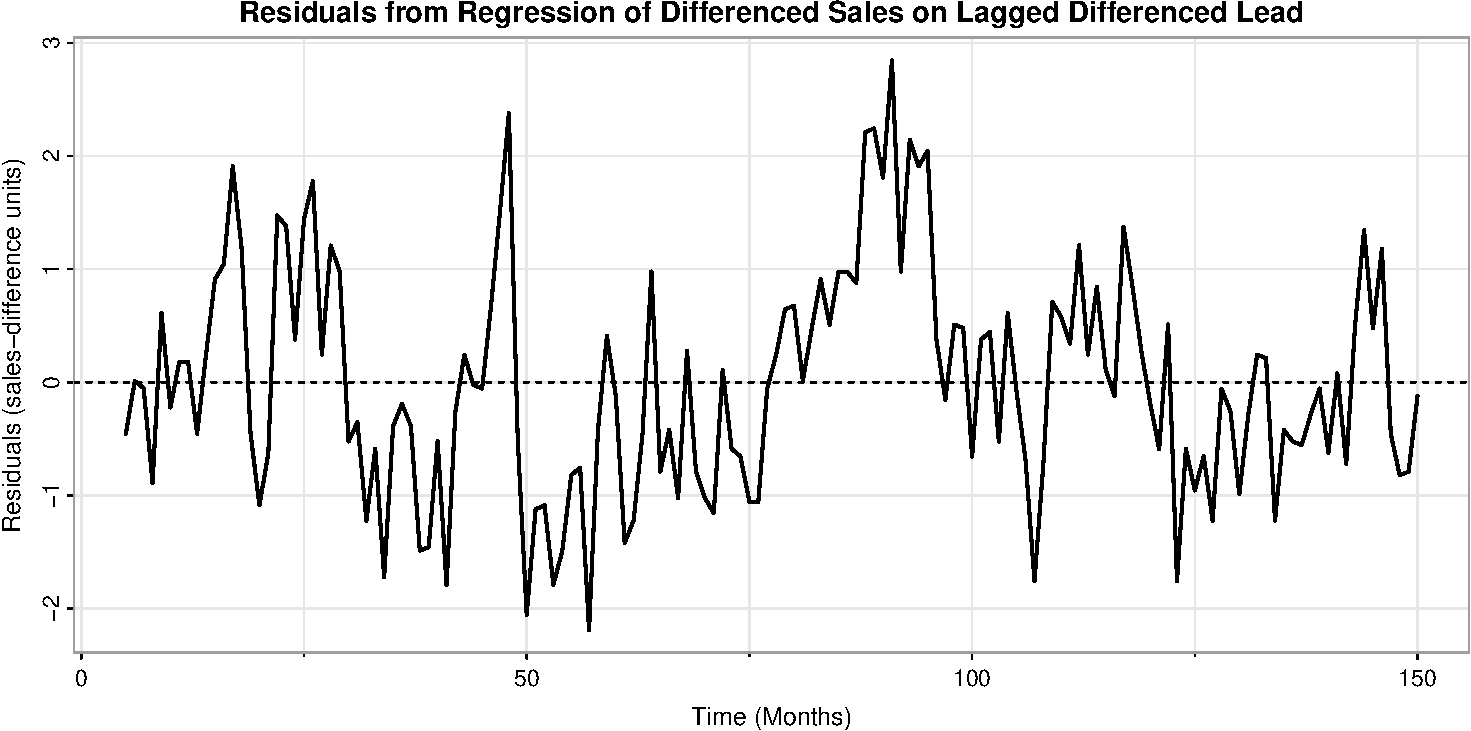
\includegraphics[width=\linewidth]{Homework4_files/figure-latex/unnamed-chunk-7-1} \end{center}

While some may be redundant with my response in part (d), the predictor is highly significant (\(p < 2 \times 10^{-16}\)), and the overall regression model is also highly significant because the F-test has \(p < 2.2 \times 10^{-16}\). The coefficient of determination is \(R^2 = 0.53\), so the model explains about 53\% of the variation in the monthly change in sales. The residual standard error is 1 in sales-difference units. This means on average, the predicted current monthly change in sales deviates from the actual current monthly change in sales by about 1 units. From the residual plot, the residuals fluctuate around zero, but they do not look completely random. There are noticeable runs of positive and negative residuals and some clustering, so the regression captures an important lagged relation but does not fully remove all dependence in the differenced sales series. Overall, the model performs reasonably well in terms of significance and \(R^2\), but the residual plot suggests that it is not the full story.

\newpage

\section{Problem 2}\label{problem-2}

\begin{problem}[Problem 2]
For your data analysis project, do the following.
\end{problem}

\begin{Shaded}
\begin{Highlighting}[]
\CommentTok{\# Load the curated data{-}project file.}
\NormalTok{blackwood\_gbgs }\OtherTok{\textless{}{-}}\NormalTok{ utils}\SpecialCharTok{::}\FunctionTok{read.csv}\NormalTok{(}
  \StringTok{\textquotesingle{}data/blackwood\_gbgs.csv\textquotesingle{}}\NormalTok{,}
  \AttributeTok{stringsAsFactors =} \ConstantTok{FALSE}
\NormalTok{)}
\end{Highlighting}
\end{Shaded}

\newpage

\subsection{Problem 2 (a)}\label{problem-2-a}

\begin{problem}[Problem 2 (a)]
Introduce your data project problem in detail explaining research goals clearly. Share your data in detail with all variables, source, and how this data was selected (that us why not another dataset).
\end{problem}

My data-analysis project asks whether a goalie's goals saved above expected, or GSAx, is really as team-independent as it is often treated in hockey analysis. The usual appeal of GSAx is that it seems fairer than raw save percentage or goals against because it does not treat all shots as equal; instead, it rewards a goalie for stopping dangerous chances and penalizes him more for allowing them, so in principle it already adjusts for the playing conditions his team gives him. I want to challenge that interpretation rather than simply accept it. My question is whether a goalie's game-by-game GSAx still moves in meaningful ways with team circumstances such as how much expected offense his team creates, how much expected danger it allows, and how much volume he faces. At the same time, I do not want to overstate the claim, because goalie performance can also vary for reasons that are not fully captured by team context, including natural progression or regression over a career, injury or recovery, confidence and mental state, fatigue, or back-to-back scheduling. So the project is not asking whether team context is the only driver of GSAx; it is asking whether team context still appears related to a metric that is usually advertised as already context-adjusted.

I will study Mackenzie Blackwood's NHL regular-season career game by game, using \(t\) as career game number so that \(t = 1, 2, \ldots, 287\), where \(t=1\) corresponds to 2018-12-18 and \(t=287\) corresponds to 2026-03-14. This version of the project is restricted to even strength, so every hockey variable in the final file is built from the GBG \texttt{\_ev} fields rather than all-situations totals. I chose this dataset because it keeps the subject fixed to one goalie, which keeps the project simple, but it still contains natural changes in team environment through Blackwood's moves from the New Jersey Devils to the San Jose Sharks and then to the Colorado Avalanche. In the final curated file, he has 152 games with New Jersey, 63 games with San Jose, and 72 games with Colorado, so the same goalie can be observed across multiple team contexts rather than comparing many different goalies at once.

The raw NHL event and report data in my broader pipeline do start with my \texttt{nhlscraper} package through functions such as \texttt{nhlscraper::games()}, \texttt{nhlscraper::goalie\_game\_report()}, \texttt{nhlscraper::gc\_pbps()}, and \texttt{nhlscraper::shift\_charts()}, but the expected-goals layer used here is not merely a direct \texttt{nhlscraper} output. In \texttt{rentosrink}, I build my own xG pipeline on top of those inputs. The current model and deployment logic are described in the live Streamlit model page at \href{https://rentosrink.streamlit.app/}{\texttt{rentosrink.streamlit.app}} and in the source file \href{https://github.com/RentoSaijo/rentosrink/blob/main/views/expected_goal.py}{\texttt{rentosrink/views/expected\_goal.py}}. The advanced game-by-game files used here are described in the GBG codebook at \href{https://github.com/RentoSaijo/rentosrink/blob/main/scripts/gbgs/codebook.md}{\texttt{rentosrink/scripts/gbgs/codebook.md}}, which states that advanced GBGs are built from the SBS/xG pipeline rather than from raw reports alone.

Because this project is restricted to even-strength data, the relevant 2025--26 unseen-future xG validation is the two even-strength partitions rather than an all-situations aggregate. For Standard 5v5, the deployed \texttt{sd1} XGBoost model achieved log loss \(= 0.1926\), Brier score \(= 0.0522\), ROC AUC \(= 0.8038\), and calibration ratio \(= 1.0477\). For Non-Standard Even Strength, the deployed \texttt{ev2} LightGBM model achieved log loss \(= 0.2986\), Brier score \(= 0.0853\), ROC AUC \(= 0.7365\), and calibration ratio \(= 1.1595\). Those numbers matter here because my project depends on the quality of the xG estimates that feed the even-strength variables \texttt{xga\_ev}, \texttt{xgf\_ev}, \texttt{gsax\_ev}, and \texttt{team\_xg\_pct\_ev}; if the xG model were poor, then the entire goalie-context question would be much weaker. At the same time, even a strong public xG model is still incomplete. In particular, the public NHL event data do not provide full pass-tracking information, so my public xG models still cannot fully account for detailed pre-shot passing structure, deception, or some off-puck context. That means if team-context variables still show a relationship with GSAx, the project may reveal not only genuine team influence on goalie results, but also what the current public xG framework is still missing.

The final project file was created by filtering the \texttt{rentosrink} goalie and team game-by-game tables in \href{https://github.com/RentoSaijo/rentosrink/tree/main/data/gbgs/basic}{\texttt{rentosrink/data/gbgs/basic}} and \href{https://github.com/RentoSaijo/rentosrink/tree/main/data/gbgs/advanced}{\texttt{rentosrink/data/gbgs/advanced}} to Blackwood's player id \texttt{8478406}, merging the goalie basic, goalie advanced, and team advanced files by game and team, joining team names from \href{https://github.com/RentoSaijo/rentosrink/blob/main/data/teams.csv}{\texttt{rentosrink/data/teams.csv}}, and keeping the even-strength columns only. The final analysis file \href{https://github.com/RentoSaijo/STA209/blob/main/data/blackwood_gbgs.csv}{\texttt{STA209/data/blackwood\_gbgs.csv}} therefore contains 287 complete observations.

The identifier and indexing variables are \texttt{game\_number}, which is the time index \(t\); \texttt{game\_date}, the calendar date of the game; \texttt{season}, the NHL season id; \texttt{team\_id}, \texttt{team\_abbr}, and \texttt{team\_name}, which identify Blackwood's team in that game; \texttt{game\_id} and \texttt{player\_id}; and \texttt{team\_change}, an indicator for the first game after a franchise change. The hockey performance variables are \texttt{shots\_against\_ev}, \texttt{goals\_against\_ev}, \texttt{xga\_ev}, \texttt{xgf\_ev}, \texttt{sv\_pct\_ev}, \texttt{gsax\_ev}, \texttt{cumulative\_gsax\_ev}, and \texttt{cumulative\_sv\_pct\_ev}. The main derived team-context variable is
\[
\texttt{team\_xg\_pct\_ev} = 100 \times \frac{\texttt{xgf\_ev}}{\texttt{xgf\_ev} + \texttt{xga\_ev}},
\]
which is the team even-strength expected-goal share percentage.

For the actual analysis, I use \texttt{cumulative\_gsax\_ev} as the response series and consider \texttt{gsax\_ev}, \texttt{sv\_pct\_ev}, and \texttt{team\_xg\_pct\_ev} as the main explanatory series. I chose this dataset instead of a larger multi-goalie panel because the assignment is easier to execute well with one clearly defined time series, and Blackwood is a good case because he has enough games, multiple team contexts, and an immediately interpretable hockey question.

\newpage

\subsection{Problem 2 (b)}\label{problem-2-b}

\begin{problem}[Problem 2 (b)]
Find three journal articles on the research topic of your interest (called background research) using Google Scholar and OneSearch to support the relevance and importance of the research questions you are exploring. Cite the background research you did and share a summary.
\end{problem}

Using Google Scholar and OneSearch, I focused on journal articles that support three separate parts of my project question: whether hockey scoring environments are context-dependent, whether expected-goals style process metrics are more informative than raw results, and whether goalkeeper-specific shot models should explicitly account for the keeper rather than treating all context as external.

\begin{itemize}
\tightlist
\item
  The first article is Lignell, Rago, and Mohr (2020), ``Analysis of goal scoring opportunities in elite male ice hockey in relation to tactical and contextual variables,'' \textit{International Journal of Performance Analysis in Sport}, 20(6), 1003--1017, \href{https://doi.org/10.1080/24748668.2020.1823161}{https://doi.org/10.1080/24748668.2020.1823161}. This article is directly relevant because it is hockey-specific and shows that the probability of scoring is affected by tactical and contextual variables, not just by a shooter-goalie duel in isolation, which supports the idea that a goalie's environment may matter when we interpret a metric like GSAx.
\item
  The second article is Mead, O'Hare, and McMenemy (2023), ``Expected goals in football: Improving model performance and demonstrating value,'' \textit{PLOS ONE}, 18(4), e0282295, \href{https://doi.org/10.1371/journal.pone.0282295}{https://doi.org/10.1371/journal.pone.0282295}. Even though it is soccer rather than hockey, it is still very relevant because it shows that expected-goals style process measures outperform traditional shot and goal counts for prediction and evaluation, which supports using xG-based team-context variables instead of relying only on goals against or wins.
\item
  The third article is De-la-Cruz-Torres, Navarro-Castro, and Ruiz-de-Alarcón-Quintero (2025), ``An Expected Goals On Target (xGOT) Model: Accounting for Goalkeeper Performance in Football,'' \textit{Big Data and Cognitive Computing}, 9(3), 64, \href{https://doi.org/10.3390/bdcc9030064}{https://doi.org/10.3390/bdcc9030064}. This article matters because it argues that traditional shot models often overlook the goalkeeper's contribution and proposes an explicitly goalkeeper-aware post-shot model, which is conceptually close to my question because GSAx is also supposed to isolate goalie performance from chance quality.
\end{itemize}

Taken together, these three articles support the importance of my project from three directions: hockey chances are shaped by context, xG-type process metrics are valuable for performance evaluation, and goalkeeper evaluation is strongest when the model takes both chance quality and the keeper's contribution seriously rather than assuming independence by default.

\newpage

\subsection{Problem 2 (c)}\label{problem-2-c}

\begin{problem}[Problem 2 (c)]
For each variable, show time series plots (you can do multiple plots on the same slide) and comment on its main features (trend, seasonality, range, volatile, heteroscedasticity). Model the trend and seasonality of all variables (at least three) using techniques learned in the class and report the best model justifying their performance using all methods learned in class. Make a summary table comparing adjusted \(R^2\), F-test, likelihood-based criteria, and forecast evaluation criteria. For seasonality, make a periodogram of your response variable (one time series) and see if there is any seasonality in the data.
\end{problem}

For this part, I focus on \texttt{cumulative\_gsax\_ev}, which is Blackwood's cumulative even-strength goals saved above expected. The other three series I use alongside it are \texttt{gsax\_ev}, the game-by-game even-strength GSAx series, \texttt{sv\_pct\_ev}, the game-by-game even-strength save-percentage series, and \texttt{team\_xg\_pct\_ev}, the team even-strength expected-goal share percentage. The time variable is the career game index \(t\), measured in games, with one observation per game from \(t=1\) on 2018-12-18 through \(t=287\) on 2026-03-14.

For forecast evaluation, I use Blackwood's move to Colorado as the forecasting cutoff, so the training sample is the pre-Colorado period \(t=1,\ldots,215\) and the holdout sample is the Colorado period \(t=216,\ldots,287\), beginning on 2024-12-14. This is a meaningful cutoff because it tests whether a model fit on Blackwood's pre-Colorado career carries into a new team environment.

\begin{Shaded}
\begin{Highlighting}[]
\CommentTok{\# Setup for the cumulative GSAx analysis.}
\NormalTok{split\_game }\OtherTok{\textless{}{-}} \FunctionTok{min}\NormalTok{(blackwood\_gbgs}\SpecialCharTok{$}\NormalTok{game\_number[blackwood\_gbgs}\SpecialCharTok{$}\NormalTok{team\_abbr }\SpecialCharTok{==} \StringTok{\textquotesingle{}COL\textquotesingle{}}\NormalTok{])}

\NormalTok{periodogram\_info }\OtherTok{\textless{}{-}} \ControlFlowTok{function}\NormalTok{(y) \{}
\NormalTok{  x }\OtherTok{\textless{}{-}}\NormalTok{ y }\SpecialCharTok{{-}} \FunctionTok{mean}\NormalTok{(y)}
\NormalTok{  n }\OtherTok{\textless{}{-}} \FunctionTok{length}\NormalTok{(x)}
\NormalTok{  I }\OtherTok{\textless{}{-}} \FunctionTok{abs}\NormalTok{(stats}\SpecialCharTok{::}\FunctionTok{fft}\NormalTok{(x))}\SpecialCharTok{\^{}}\DecValTok{2} \SpecialCharTok{/}\NormalTok{ n}
\NormalTok{  half }\OtherTok{\textless{}{-}} \FunctionTok{floor}\NormalTok{((n }\SpecialCharTok{/} \DecValTok{2}\NormalTok{) }\SpecialCharTok{{-}} \DecValTok{1}\NormalTok{)}
\NormalTok{  f }\OtherTok{\textless{}{-}} \DecValTok{0}\SpecialCharTok{:}\NormalTok{half }\SpecialCharTok{/}\NormalTok{ n}
\NormalTok{  P }\OtherTok{\textless{}{-}}\NormalTok{ (}\DecValTok{4} \SpecialCharTok{/}\NormalTok{ n) }\SpecialCharTok{*}\NormalTok{ I[}\DecValTok{1}\SpecialCharTok{:}\NormalTok{(half }\SpecialCharTok{+} \DecValTok{1}\NormalTok{)]}
\NormalTok{  dom\_idx }\OtherTok{\textless{}{-}} \FunctionTok{which.max}\NormalTok{(P[}\SpecialCharTok{{-}}\DecValTok{1}\NormalTok{]) }\SpecialCharTok{+} \DecValTok{1}
  \FunctionTok{list}\NormalTok{(}\AttributeTok{f =}\NormalTok{ f, }\AttributeTok{P =}\NormalTok{ P, }\AttributeTok{freq =}\NormalTok{ f[dom\_idx], }\AttributeTok{period =} \DecValTok{1} \SpecialCharTok{/}\NormalTok{ f[dom\_idx])}
\NormalTok{\}}

\NormalTok{acf\_table }\OtherTok{\textless{}{-}} \ControlFlowTok{function}\NormalTok{(x, }\AttributeTok{lag.max =} \DecValTok{8}\NormalTok{) \{}
\NormalTok{  ac }\OtherTok{\textless{}{-}}\NormalTok{ stats}\SpecialCharTok{::}\FunctionTok{acf}\NormalTok{(}\FunctionTok{as.numeric}\NormalTok{(x), }\AttributeTok{lag.max =}\NormalTok{ lag.max, }\AttributeTok{plot =} \ConstantTok{FALSE}\NormalTok{)}
  \FunctionTok{data.frame}\NormalTok{(}\AttributeTok{lag =} \FunctionTok{as.numeric}\NormalTok{(ac}\SpecialCharTok{$}\NormalTok{lag)[}\SpecialCharTok{{-}}\DecValTok{1}\NormalTok{], }\AttributeTok{acf =} \FunctionTok{as.numeric}\NormalTok{(ac}\SpecialCharTok{$}\NormalTok{acf)[}\SpecialCharTok{{-}}\DecValTok{1}\NormalTok{])}
\NormalTok{\}}

\NormalTok{ccf\_table }\OtherTok{\textless{}{-}} \ControlFlowTok{function}\NormalTok{(x, y, }\AttributeTok{lag.max =} \DecValTok{8}\NormalTok{) \{}
\NormalTok{  cc }\OtherTok{\textless{}{-}}\NormalTok{ stats}\SpecialCharTok{::}\FunctionTok{ccf}\NormalTok{(}\FunctionTok{as.numeric}\NormalTok{(x), }\FunctionTok{as.numeric}\NormalTok{(y), }\AttributeTok{lag.max =}\NormalTok{ lag.max, }\AttributeTok{plot =} \ConstantTok{FALSE}\NormalTok{)}
  \FunctionTok{data.frame}\NormalTok{(}\AttributeTok{lag =} \FunctionTok{as.numeric}\NormalTok{(cc}\SpecialCharTok{$}\NormalTok{lag), }\AttributeTok{acf =} \FunctionTok{as.numeric}\NormalTok{(cc}\SpecialCharTok{$}\NormalTok{acf))}
\NormalTok{\}}

\NormalTok{neg\_lag\_peak }\OtherTok{\textless{}{-}} \ControlFlowTok{function}\NormalTok{(tbl) \{}
\NormalTok{  tbl }\OtherTok{\textless{}{-}}\NormalTok{ tbl[tbl}\SpecialCharTok{$}\NormalTok{lag }\SpecialCharTok{\textless{}} \DecValTok{0}\NormalTok{, , drop }\OtherTok{=} \ConstantTok{FALSE}\NormalTok{]}
\NormalTok{  tbl[}\FunctionTok{which.max}\NormalTok{(}\FunctionTok{abs}\NormalTok{(tbl}\SpecialCharTok{$}\NormalTok{acf)), ]}
\NormalTok{\}}

\NormalTok{fit\_table\_proj }\OtherTok{\textless{}{-}} \ControlFlowTok{function}\NormalTok{(fit) \{}
\NormalTok{  n }\OtherTok{\textless{}{-}} \FunctionTok{length}\NormalTok{(stats}\SpecialCharTok{::}\FunctionTok{residuals}\NormalTok{(fit))}
\NormalTok{  r }\OtherTok{\textless{}{-}} \FunctionTok{length}\NormalTok{(stats}\SpecialCharTok{::}\FunctionTok{coef}\NormalTok{(fit))}
\NormalTok{  sse }\OtherTok{\textless{}{-}} \FunctionTok{sum}\NormalTok{(stats}\SpecialCharTok{::}\FunctionTok{residuals}\NormalTok{(fit)}\SpecialCharTok{\^{}}\DecValTok{2}\NormalTok{)}
\NormalTok{  f\_stats }\OtherTok{\textless{}{-}} \FunctionTok{summary}\NormalTok{(fit)}\SpecialCharTok{$}\NormalTok{fstatistic}
\NormalTok{  f\_p }\OtherTok{\textless{}{-}}\NormalTok{ stats}\SpecialCharTok{::}\FunctionTok{pf}\NormalTok{(f\_stats[}\DecValTok{1}\NormalTok{], f\_stats[}\DecValTok{2}\NormalTok{], f\_stats[}\DecValTok{3}\NormalTok{], }\AttributeTok{lower.tail =} \ConstantTok{FALSE}\NormalTok{)}
  \FunctionTok{data.frame}\NormalTok{(}
    \AttributeTok{Parameters =}\NormalTok{ r,}
    \AttributeTok{R2a =} \FunctionTok{summary}\NormalTok{(fit)}\SpecialCharTok{$}\NormalTok{adj.r.squared,}
    \AttributeTok{Fp =}\NormalTok{ f\_p,}
    \AttributeTok{AIC =}\NormalTok{ stats}\SpecialCharTok{::}\FunctionTok{AIC}\NormalTok{(fit) }\SpecialCharTok{/}\NormalTok{ n,}
    \AttributeTok{AICC =} \FunctionTok{log}\NormalTok{(sse }\SpecialCharTok{/}\NormalTok{ n) }\SpecialCharTok{+}\NormalTok{ ((n }\SpecialCharTok{+}\NormalTok{ r) }\SpecialCharTok{/}\NormalTok{ (n }\SpecialCharTok{{-}}\NormalTok{ r }\SpecialCharTok{{-}} \DecValTok{2}\NormalTok{)),}
    \AttributeTok{BIC =}\NormalTok{ stats}\SpecialCharTok{::}\FunctionTok{AIC}\NormalTok{(fit, }\AttributeTok{k =} \FunctionTok{log}\NormalTok{(n)) }\SpecialCharTok{/}\NormalTok{ n,}
    \AttributeTok{row.names =} \ConstantTok{NULL}
\NormalTok{  )}
\NormalTok{\}}

\NormalTok{fcst\_metrics\_proj }\OtherTok{\textless{}{-}} \ControlFlowTok{function}\NormalTok{(data, form) \{}
\NormalTok{  train\_data }\OtherTok{\textless{}{-}}\NormalTok{ data[data}\SpecialCharTok{$}\NormalTok{t }\SpecialCharTok{\textless{}}\NormalTok{ split\_game, , drop }\OtherTok{=} \ConstantTok{FALSE}\NormalTok{]}
\NormalTok{  test\_data }\OtherTok{\textless{}{-}}\NormalTok{ data[data}\SpecialCharTok{$}\NormalTok{t }\SpecialCharTok{\textgreater{}=}\NormalTok{ split\_game, , drop }\OtherTok{=} \ConstantTok{FALSE}\NormalTok{]}
\NormalTok{  fit\_train }\OtherTok{\textless{}{-}}\NormalTok{ stats}\SpecialCharTok{::}\FunctionTok{lm}\NormalTok{(form, }\AttributeTok{data =}\NormalTok{ train\_data)}
\NormalTok{  y\_hat }\OtherTok{\textless{}{-}}\NormalTok{ stats}\SpecialCharTok{::}\FunctionTok{predict}\NormalTok{(fit\_train, }\AttributeTok{newdata =}\NormalTok{ test\_data)}
\NormalTok{  e }\OtherTok{\textless{}{-}}\NormalTok{ test\_data}\SpecialCharTok{$}\NormalTok{H }\SpecialCharTok{{-}}\NormalTok{ y\_hat}
  \FunctionTok{data.frame}\NormalTok{(}
    \AttributeTok{ME =} \FunctionTok{mean}\NormalTok{(e),}
    \AttributeTok{MPE =} \DecValTok{100} \SpecialCharTok{*} \FunctionTok{mean}\NormalTok{(e }\SpecialCharTok{/}\NormalTok{ test\_data}\SpecialCharTok{$}\NormalTok{H),}
    \AttributeTok{MSE =} \FunctionTok{mean}\NormalTok{(e}\SpecialCharTok{\^{}}\DecValTok{2}\NormalTok{),}
    \AttributeTok{MAE =} \FunctionTok{mean}\NormalTok{(}\FunctionTok{abs}\NormalTok{(e)),}
    \AttributeTok{MAPE =} \DecValTok{100} \SpecialCharTok{*} \FunctionTok{mean}\NormalTok{(}\FunctionTok{abs}\NormalTok{(e }\SpecialCharTok{/}\NormalTok{ test\_data}\SpecialCharTok{$}\NormalTok{H)),}
    \AttributeTok{row.names =} \ConstantTok{NULL}
\NormalTok{  )}
\NormalTok{\}}

\NormalTok{H }\OtherTok{\textless{}{-}}\NormalTok{ stats}\SpecialCharTok{::}\FunctionTok{ts}\NormalTok{(blackwood\_gbgs}\SpecialCharTok{$}\NormalTok{cumulative\_gsax\_ev, }\AttributeTok{start =} \DecValTok{1}\NormalTok{, }\AttributeTok{frequency =} \DecValTok{1}\NormalTok{)}
\NormalTok{G }\OtherTok{\textless{}{-}}\NormalTok{ stats}\SpecialCharTok{::}\FunctionTok{ts}\NormalTok{(blackwood\_gbgs}\SpecialCharTok{$}\NormalTok{gsax\_ev, }\AttributeTok{start =} \DecValTok{1}\NormalTok{, }\AttributeTok{frequency =} \DecValTok{1}\NormalTok{)}
\NormalTok{S }\OtherTok{\textless{}{-}}\NormalTok{ stats}\SpecialCharTok{::}\FunctionTok{ts}\NormalTok{(blackwood\_gbgs}\SpecialCharTok{$}\NormalTok{sv\_pct\_ev, }\AttributeTok{start =} \DecValTok{1}\NormalTok{, }\AttributeTok{frequency =} \DecValTok{1}\NormalTok{)}
\NormalTok{X }\OtherTok{\textless{}{-}}\NormalTok{ stats}\SpecialCharTok{::}\FunctionTok{ts}\NormalTok{(blackwood\_gbgs}\SpecialCharTok{$}\NormalTok{team\_xg\_pct\_ev, }\AttributeTok{start =} \DecValTok{1}\NormalTok{, }\AttributeTok{frequency =} \DecValTok{1}\NormalTok{)}
\NormalTok{t }\OtherTok{\textless{}{-}}\NormalTok{ stats}\SpecialCharTok{::}\FunctionTok{ts}\NormalTok{(}\DecValTok{1}\SpecialCharTok{:}\FunctionTok{length}\NormalTok{(H), }\AttributeTok{start =} \DecValTok{1}\NormalTok{, }\AttributeTok{frequency =} \DecValTok{1}\NormalTok{)}
\NormalTok{t2 }\OtherTok{\textless{}{-}}\NormalTok{ stats}\SpecialCharTok{::}\FunctionTok{ts}\NormalTok{((}\DecValTok{1}\SpecialCharTok{:}\FunctionTok{length}\NormalTok{(H))}\SpecialCharTok{\^{}}\DecValTok{2} \SpecialCharTok{/} \FunctionTok{factorial}\NormalTok{(}\DecValTok{2}\NormalTok{), }\AttributeTok{start =} \DecValTok{1}\NormalTok{, }\AttributeTok{frequency =} \DecValTok{1}\NormalTok{)}
\NormalTok{t3 }\OtherTok{\textless{}{-}}\NormalTok{ stats}\SpecialCharTok{::}\FunctionTok{ts}\NormalTok{((}\DecValTok{1}\SpecialCharTok{:}\FunctionTok{length}\NormalTok{(H))}\SpecialCharTok{\^{}}\DecValTok{3} \SpecialCharTok{/} \FunctionTok{factorial}\NormalTok{(}\DecValTok{3}\NormalTok{), }\AttributeTok{start =} \DecValTok{1}\NormalTok{, }\AttributeTok{frequency =} \DecValTok{1}\NormalTok{)}

\NormalTok{gsax\_data }\OtherTok{\textless{}{-}}\NormalTok{ stats}\SpecialCharTok{::}\FunctionTok{ts.intersect}\NormalTok{(}
  \AttributeTok{H =}\NormalTok{ H,}
  \AttributeTok{t =}\NormalTok{ t,}
  \AttributeTok{t2 =}\NormalTok{ t2,}
  \AttributeTok{t3 =}\NormalTok{ t3,}
  \AttributeTok{GL3 =}\NormalTok{ stats}\SpecialCharTok{::}\FunctionTok{lag}\NormalTok{(G, }\SpecialCharTok{{-}}\DecValTok{3}\NormalTok{),}
  \AttributeTok{SL3 =}\NormalTok{ stats}\SpecialCharTok{::}\FunctionTok{lag}\NormalTok{(S, }\SpecialCharTok{{-}}\DecValTok{3}\NormalTok{),}
  \AttributeTok{dframe =} \ConstantTok{TRUE}
\NormalTok{)}

\NormalTok{gsax\_period }\OtherTok{\textless{}{-}} \FunctionTok{periodogram\_info}\NormalTok{(blackwood\_gbgs}\SpecialCharTok{$}\NormalTok{cumulative\_gsax\_ev)}
\NormalTok{h\_acf\_tbl }\OtherTok{\textless{}{-}} \FunctionTok{acf\_table}\NormalTok{(blackwood\_gbgs}\SpecialCharTok{$}\NormalTok{cumulative\_gsax\_ev)}
\NormalTok{g\_ccf\_tbl }\OtherTok{\textless{}{-}} \FunctionTok{ccf\_table}\NormalTok{(blackwood\_gbgs}\SpecialCharTok{$}\NormalTok{gsax\_ev, blackwood\_gbgs}\SpecialCharTok{$}\NormalTok{cumulative\_gsax\_ev)}
\NormalTok{s\_ccf\_tbl }\OtherTok{\textless{}{-}} \FunctionTok{ccf\_table}\NormalTok{(blackwood\_gbgs}\SpecialCharTok{$}\NormalTok{sv\_pct\_ev, blackwood\_gbgs}\SpecialCharTok{$}\NormalTok{cumulative\_gsax\_ev)}
\NormalTok{x\_ccf\_tbl }\OtherTok{\textless{}{-}} \FunctionTok{ccf\_table}\NormalTok{(blackwood\_gbgs}\SpecialCharTok{$}\NormalTok{team\_xg\_pct\_ev, blackwood\_gbgs}\SpecialCharTok{$}\NormalTok{cumulative\_gsax\_ev)}

\NormalTok{g\_ccf\_neg }\OtherTok{\textless{}{-}} \FunctionTok{neg\_lag\_peak}\NormalTok{(g\_ccf\_tbl)}
\NormalTok{s\_ccf\_neg }\OtherTok{\textless{}{-}} \FunctionTok{neg\_lag\_peak}\NormalTok{(s\_ccf\_tbl)}
\NormalTok{x\_ccf\_neg }\OtherTok{\textless{}{-}} \FunctionTok{neg\_lag\_peak}\NormalTok{(x\_ccf\_tbl)}
\end{Highlighting}
\end{Shaded}

\begin{Shaded}
\begin{Highlighting}[]
\CommentTok{\# Time series plots for the response and candidate predictors.}
\NormalTok{op }\OtherTok{\textless{}{-}}\NormalTok{ graphics}\SpecialCharTok{::}\FunctionTok{par}\NormalTok{(}\AttributeTok{no.readonly =} \ConstantTok{TRUE}\NormalTok{)}
\FunctionTok{on.exit}\NormalTok{(graphics}\SpecialCharTok{::}\FunctionTok{par}\NormalTok{(op), }\AttributeTok{add =} \ConstantTok{TRUE}\NormalTok{)}
\NormalTok{graphics}\SpecialCharTok{::}\FunctionTok{par}\NormalTok{(}\AttributeTok{mfrow =} \FunctionTok{c}\NormalTok{(}\DecValTok{2}\NormalTok{, }\DecValTok{2}\NormalTok{))}
\NormalTok{astsa}\SpecialCharTok{::}\FunctionTok{tsplot}\NormalTok{(}
\NormalTok{  stats}\SpecialCharTok{::}\FunctionTok{ts}\NormalTok{(blackwood\_gbgs}\SpecialCharTok{$}\NormalTok{cumulative\_gsax\_ev, }\AttributeTok{start =} \DecValTok{1}\NormalTok{, }\AttributeTok{frequency =} \DecValTok{1}\NormalTok{),}
  \AttributeTok{main =} \StringTok{\textquotesingle{}Even{-}Strength Cumulative GSAx\textquotesingle{}}\NormalTok{,}
  \AttributeTok{xlab =} \StringTok{\textquotesingle{}Career Game Number (t)\textquotesingle{}}\NormalTok{,}
  \AttributeTok{ylab =} \StringTok{\textquotesingle{}Cumulative GSAx at EV (Goals)\textquotesingle{}}\NormalTok{,}
  \AttributeTok{col =} \StringTok{\textquotesingle{}darkgreen\textquotesingle{}}\NormalTok{,}
  \AttributeTok{lwd =} \DecValTok{2}
\NormalTok{)}
\NormalTok{astsa}\SpecialCharTok{::}\FunctionTok{tsplot}\NormalTok{(}
\NormalTok{  stats}\SpecialCharTok{::}\FunctionTok{ts}\NormalTok{(blackwood\_gbgs}\SpecialCharTok{$}\NormalTok{gsax\_ev, }\AttributeTok{start =} \DecValTok{1}\NormalTok{, }\AttributeTok{frequency =} \DecValTok{1}\NormalTok{),}
  \AttributeTok{main =} \StringTok{\textquotesingle{}Even{-}Strength Game{-}by{-}Game GSAx\textquotesingle{}}\NormalTok{,}
  \AttributeTok{xlab =} \StringTok{\textquotesingle{}Career Game Number (t)\textquotesingle{}}\NormalTok{,}
  \AttributeTok{ylab =} \StringTok{\textquotesingle{}GSAx at EV (Goals)\textquotesingle{}}\NormalTok{,}
  \AttributeTok{col =} \StringTok{\textquotesingle{}firebrick\textquotesingle{}}\NormalTok{,}
  \AttributeTok{lwd =} \DecValTok{2}
\NormalTok{)}
\NormalTok{astsa}\SpecialCharTok{::}\FunctionTok{tsplot}\NormalTok{(}
\NormalTok{  stats}\SpecialCharTok{::}\FunctionTok{ts}\NormalTok{(blackwood\_gbgs}\SpecialCharTok{$}\NormalTok{sv\_pct\_ev, }\AttributeTok{start =} \DecValTok{1}\NormalTok{, }\AttributeTok{frequency =} \DecValTok{1}\NormalTok{),}
  \AttributeTok{main =} \StringTok{\textquotesingle{}Even{-}Strength Game{-}by{-}Game Save Percentage\textquotesingle{}}\NormalTok{,}
  \AttributeTok{xlab =} \StringTok{\textquotesingle{}Career Game Number (t)\textquotesingle{}}\NormalTok{,}
  \AttributeTok{ylab =} \StringTok{\textquotesingle{}SV\% at EV\textquotesingle{}}\NormalTok{,}
  \AttributeTok{col =} \StringTok{\textquotesingle{}purple4\textquotesingle{}}\NormalTok{,}
  \AttributeTok{lwd =} \DecValTok{2}
\NormalTok{)}
\NormalTok{astsa}\SpecialCharTok{::}\FunctionTok{tsplot}\NormalTok{(}
\NormalTok{  stats}\SpecialCharTok{::}\FunctionTok{ts}\NormalTok{(blackwood\_gbgs}\SpecialCharTok{$}\NormalTok{team\_xg\_pct\_ev, }\AttributeTok{start =} \DecValTok{1}\NormalTok{, }\AttributeTok{frequency =} \DecValTok{1}\NormalTok{),}
  \AttributeTok{main =} \StringTok{\textquotesingle{}Team Even{-}Strength xGF\%\textquotesingle{}}\NormalTok{,}
  \AttributeTok{xlab =} \StringTok{\textquotesingle{}Career Game Number (t)\textquotesingle{}}\NormalTok{,}
  \AttributeTok{ylab =} \StringTok{\textquotesingle{}Team xGF\% at EV (Percent)\textquotesingle{}}\NormalTok{,}
  \AttributeTok{col =} \StringTok{\textquotesingle{}navy\textquotesingle{}}\NormalTok{,}
  \AttributeTok{lwd =} \DecValTok{2}
\NormalTok{)}
\end{Highlighting}
\end{Shaded}

\begin{center}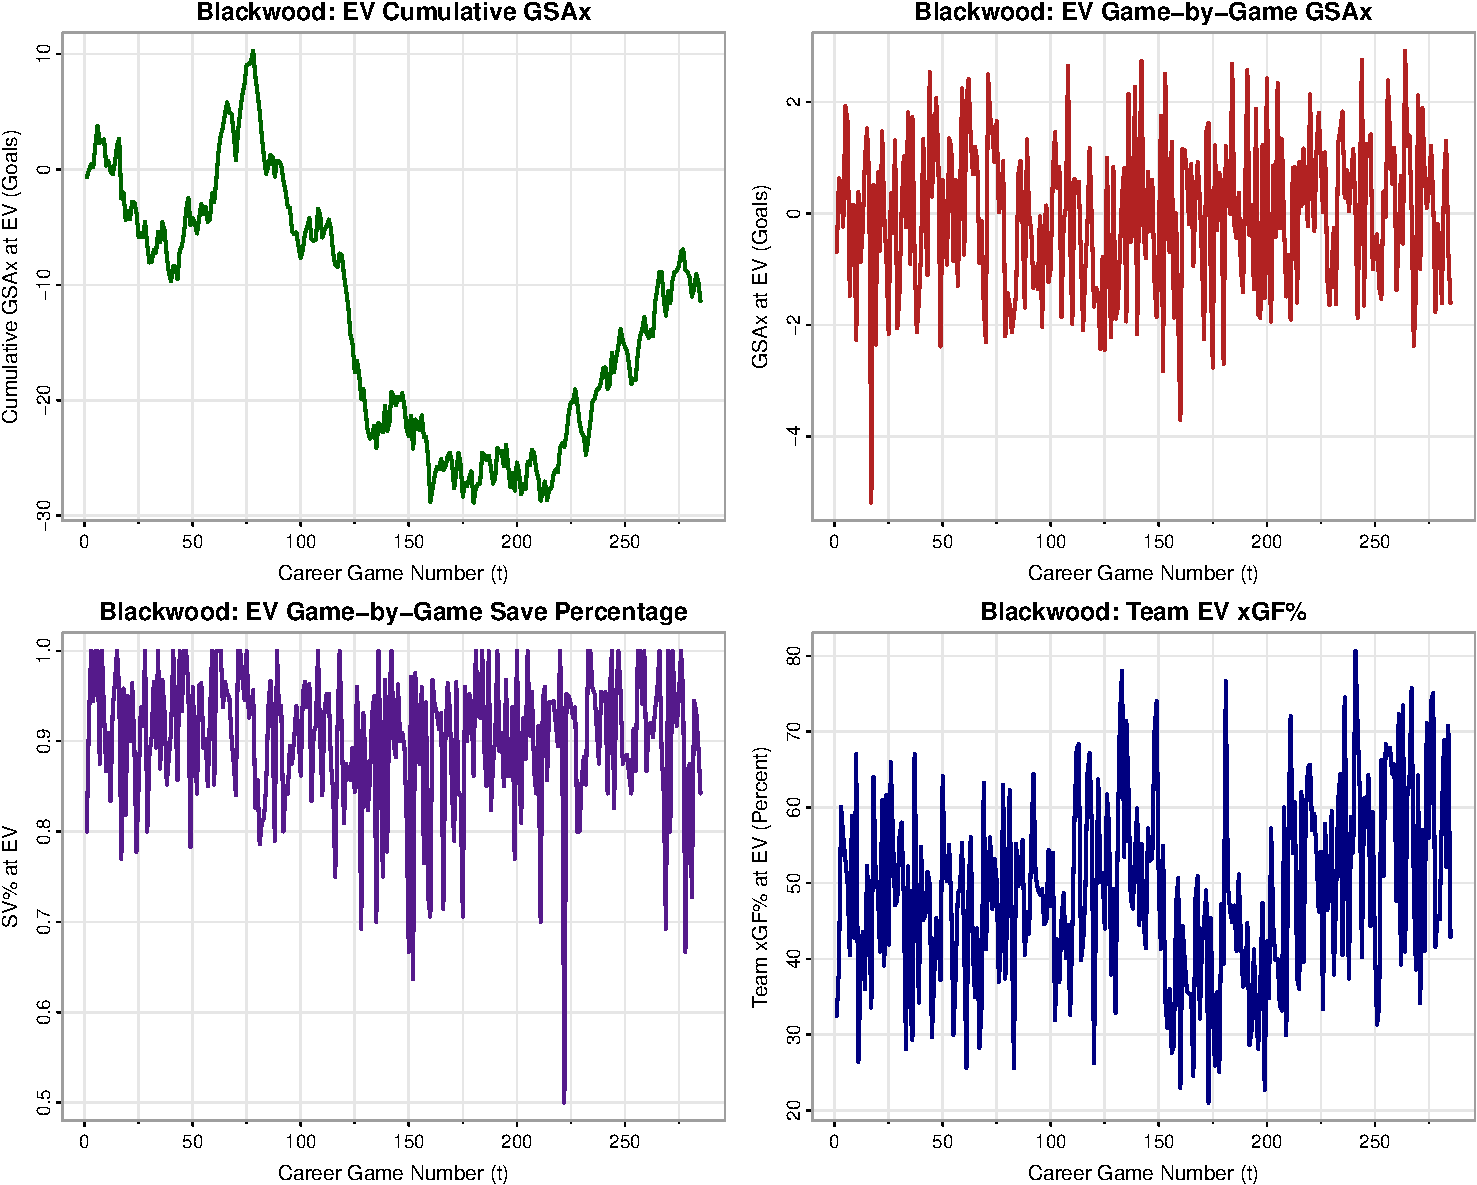
\includegraphics[width=\linewidth]{Homework4_files/figure-latex/unnamed-chunk-10-1} \end{center}

\begin{itemize}
\item
  The \texttt{cumulative\_gsax\_ev} data is Blackwood's running even-strength goals saved above expected over 287 career games. Its mean behavior is clearly time-dependent and non-linear, since the series rises early, declines for a long middle stretch, and then recovers later. There is no visible repeated seasonal pattern. Its statistical range is \(\max(H_t) - \min(H_t) = 39.145\) goals. Because the series is cumulative, its spread changes gradually rather than abruptly, and there is no strong evidence of heteroscedastic fanning or short-run volatility clustering.
\item
  The \texttt{gsax\_ev} data is Blackwood's game-by-game even-strength goals saved above expected in goals. The series fluctuates around a roughly stable center rather than showing a strong long-run deterministic trend, although there are stretches of better and worse results. There is again no visible repeated seasonal pattern. Its statistical range is \(\max(G_t) - \min(G_t) = 8.111\) goals. The variance looks fairly stable over time, so it appears approximately homoskedastic, but there are several isolated positive and negative spikes, so the game-by-game series is clearly more volatile than the cumulative series.
\item
  The \texttt{sv\_pct\_ev} data is Blackwood's game-by-game even-strength save percentage in proportion form. Like \texttt{gsax\_ev}, it fluctuates around a fairly stable mean rather than showing a clear deterministic trend, and there is no visible repeated seasonal pattern. Its statistical range is \(\max(S_t) - \min(S_t) = 0.5\). The spread looks broadly stable over the sample, so there is no strong visual evidence of heteroscedasticity. It does show occasional sharp single-game jumps, including several very strong and very weak save-percentage games, so it is moderately volatile in the short run.
\item
  The \texttt{team\_xg\_pct\_ev} data is Blackwood's team even-strength expected-goal share percentage, measured in percentage points, over the same 287 career games. Its mean behavior is time-dependent, but not in a smooth polynomial way; instead, it shows regime changes that line up more naturally with team context changes. There is no clear repeated seasonal pattern. Its statistical range is \(\max(X_t) - \min(X_t) = 71.427\) percentage points. The spread looks fairly stable over time, so it appears approximately homoskedastic, and while it does move sharply at times, it is not strongly volatile in the same spike-like way as the two game-by-game goalie-performance series.
\end{itemize}

\begin{Shaded}
\begin{Highlighting}[]
\CommentTok{\# Periodogram for cumulative GSAx at even strength.}
\NormalTok{graphics}\SpecialCharTok{::}\FunctionTok{plot}\NormalTok{(}
\NormalTok{  gsax\_period}\SpecialCharTok{$}\NormalTok{f,}
\NormalTok{  gsax\_period}\SpecialCharTok{$}\NormalTok{P,}
  \AttributeTok{type =} \StringTok{\textquotesingle{}l\textquotesingle{}}\NormalTok{,}
  \AttributeTok{main =} \StringTok{\textquotesingle{}Periodogram for cumulative\_gsax\_ev\textquotesingle{}}\NormalTok{,}
  \AttributeTok{xlab =} \StringTok{\textquotesingle{}Frequency\textquotesingle{}}\NormalTok{,}
  \AttributeTok{ylab =} \StringTok{\textquotesingle{}P(frequency)\textquotesingle{}}\NormalTok{,}
  \AttributeTok{col =} \StringTok{\textquotesingle{}navy\textquotesingle{}}\NormalTok{,}
  \AttributeTok{lwd =} \DecValTok{2}
\NormalTok{)}
\NormalTok{graphics}\SpecialCharTok{::}\FunctionTok{abline}\NormalTok{(}\AttributeTok{v =}\NormalTok{ gsax\_period}\SpecialCharTok{$}\NormalTok{freq, }\AttributeTok{col =} \StringTok{\textquotesingle{}red\textquotesingle{}}\NormalTok{, }\AttributeTok{lty =} \DecValTok{2}\NormalTok{, }\AttributeTok{lwd =} \DecValTok{2}\NormalTok{)}
\end{Highlighting}
\end{Shaded}

\begin{center}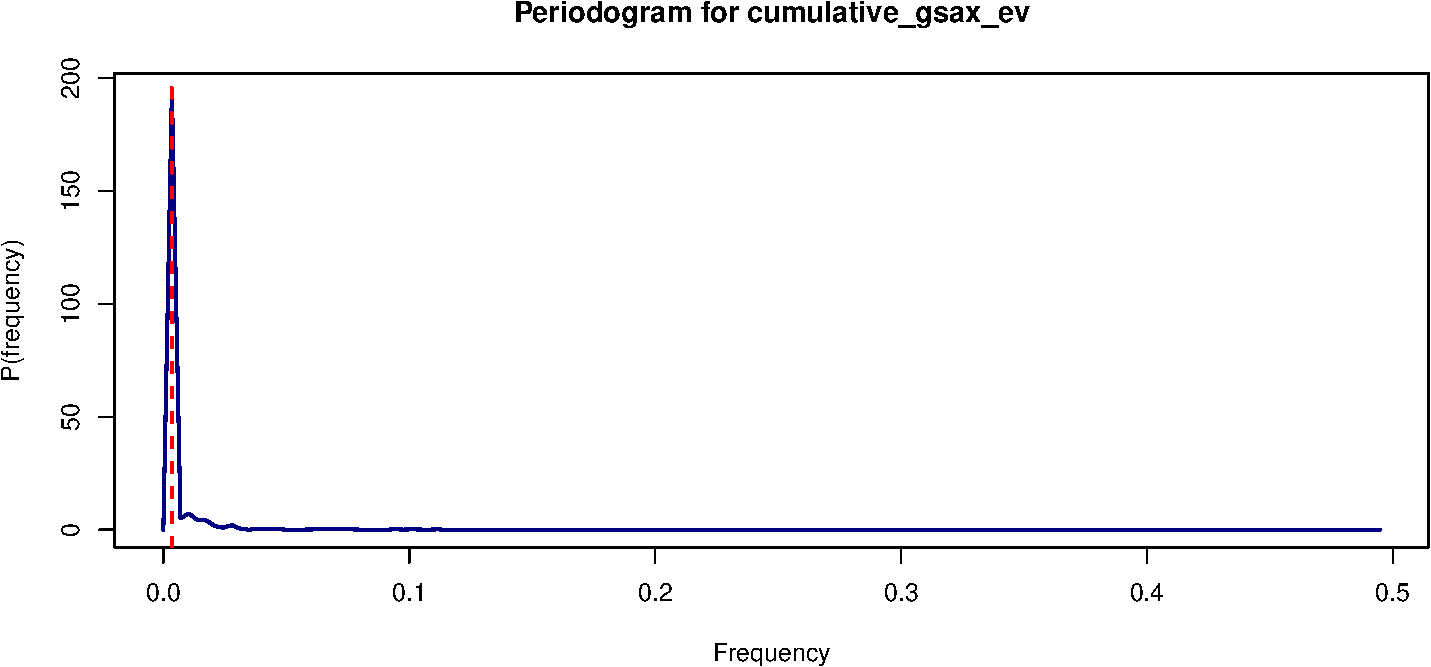
\includegraphics[width=\linewidth]{Homework4_files/figure-latex/unnamed-chunk-11-1} \end{center}

The periodogram for \texttt{cumulative\_gsax\_ev} has its dominant peak at frequency \(f = 0.003484\), which corresponds to an implied period of about 287 games. Since that period is essentially the full sample length, it reflects long-run trend rather than practical seasonality. So based on the periodogram, I do not include any seasonal harmonic or indicator terms in the candidate models.

\begin{Shaded}
\begin{Highlighting}[]
\CommentTok{\# ACF and CCF diagnostics for the cumulative response.}
\NormalTok{op }\OtherTok{\textless{}{-}}\NormalTok{ graphics}\SpecialCharTok{::}\FunctionTok{par}\NormalTok{(}\AttributeTok{no.readonly =} \ConstantTok{TRUE}\NormalTok{)}
\FunctionTok{on.exit}\NormalTok{(graphics}\SpecialCharTok{::}\FunctionTok{par}\NormalTok{(op), }\AttributeTok{add =} \ConstantTok{TRUE}\NormalTok{)}
\NormalTok{graphics}\SpecialCharTok{::}\FunctionTok{par}\NormalTok{(}\AttributeTok{mfrow =} \FunctionTok{c}\NormalTok{(}\DecValTok{2}\NormalTok{, }\DecValTok{2}\NormalTok{))}
\NormalTok{stats}\SpecialCharTok{::}\FunctionTok{acf}\NormalTok{(blackwood\_gbgs}\SpecialCharTok{$}\NormalTok{cumulative\_gsax\_ev, }\AttributeTok{lag.max =} \DecValTok{8}\NormalTok{, }\AttributeTok{main =} \StringTok{\textquotesingle{}ACF: cumulative\_gsax\_ev\textquotesingle{}}\NormalTok{)}
\NormalTok{stats}\SpecialCharTok{::}\FunctionTok{ccf}\NormalTok{(}
  \FunctionTok{as.numeric}\NormalTok{(blackwood\_gbgs}\SpecialCharTok{$}\NormalTok{gsax\_ev),}
  \FunctionTok{as.numeric}\NormalTok{(blackwood\_gbgs}\SpecialCharTok{$}\NormalTok{cumulative\_gsax\_ev),}
  \AttributeTok{lag.max =} \DecValTok{8}\NormalTok{,}
  \AttributeTok{main =} \StringTok{\textquotesingle{}CCF: gsax\_ev vs cumulative\_gsax\_ev\textquotesingle{}}
\NormalTok{)}
\NormalTok{stats}\SpecialCharTok{::}\FunctionTok{ccf}\NormalTok{(}
  \FunctionTok{as.numeric}\NormalTok{(blackwood\_gbgs}\SpecialCharTok{$}\NormalTok{sv\_pct\_ev),}
  \FunctionTok{as.numeric}\NormalTok{(blackwood\_gbgs}\SpecialCharTok{$}\NormalTok{cumulative\_gsax\_ev),}
  \AttributeTok{lag.max =} \DecValTok{8}\NormalTok{,}
  \AttributeTok{main =} \StringTok{\textquotesingle{}CCF: sv\_pct\_ev vs cumulative\_gsax\_ev\textquotesingle{}}
\NormalTok{)}
\NormalTok{stats}\SpecialCharTok{::}\FunctionTok{ccf}\NormalTok{(}
  \FunctionTok{as.numeric}\NormalTok{(blackwood\_gbgs}\SpecialCharTok{$}\NormalTok{team\_xg\_pct\_ev),}
  \FunctionTok{as.numeric}\NormalTok{(blackwood\_gbgs}\SpecialCharTok{$}\NormalTok{cumulative\_gsax\_ev),}
  \AttributeTok{lag.max =} \DecValTok{8}\NormalTok{,}
  \AttributeTok{main =} \StringTok{\textquotesingle{}CCF: team\_xg\_pct\_ev vs cumulative\_gsax\_ev\textquotesingle{}}
\NormalTok{)}
\end{Highlighting}
\end{Shaded}

\begin{center}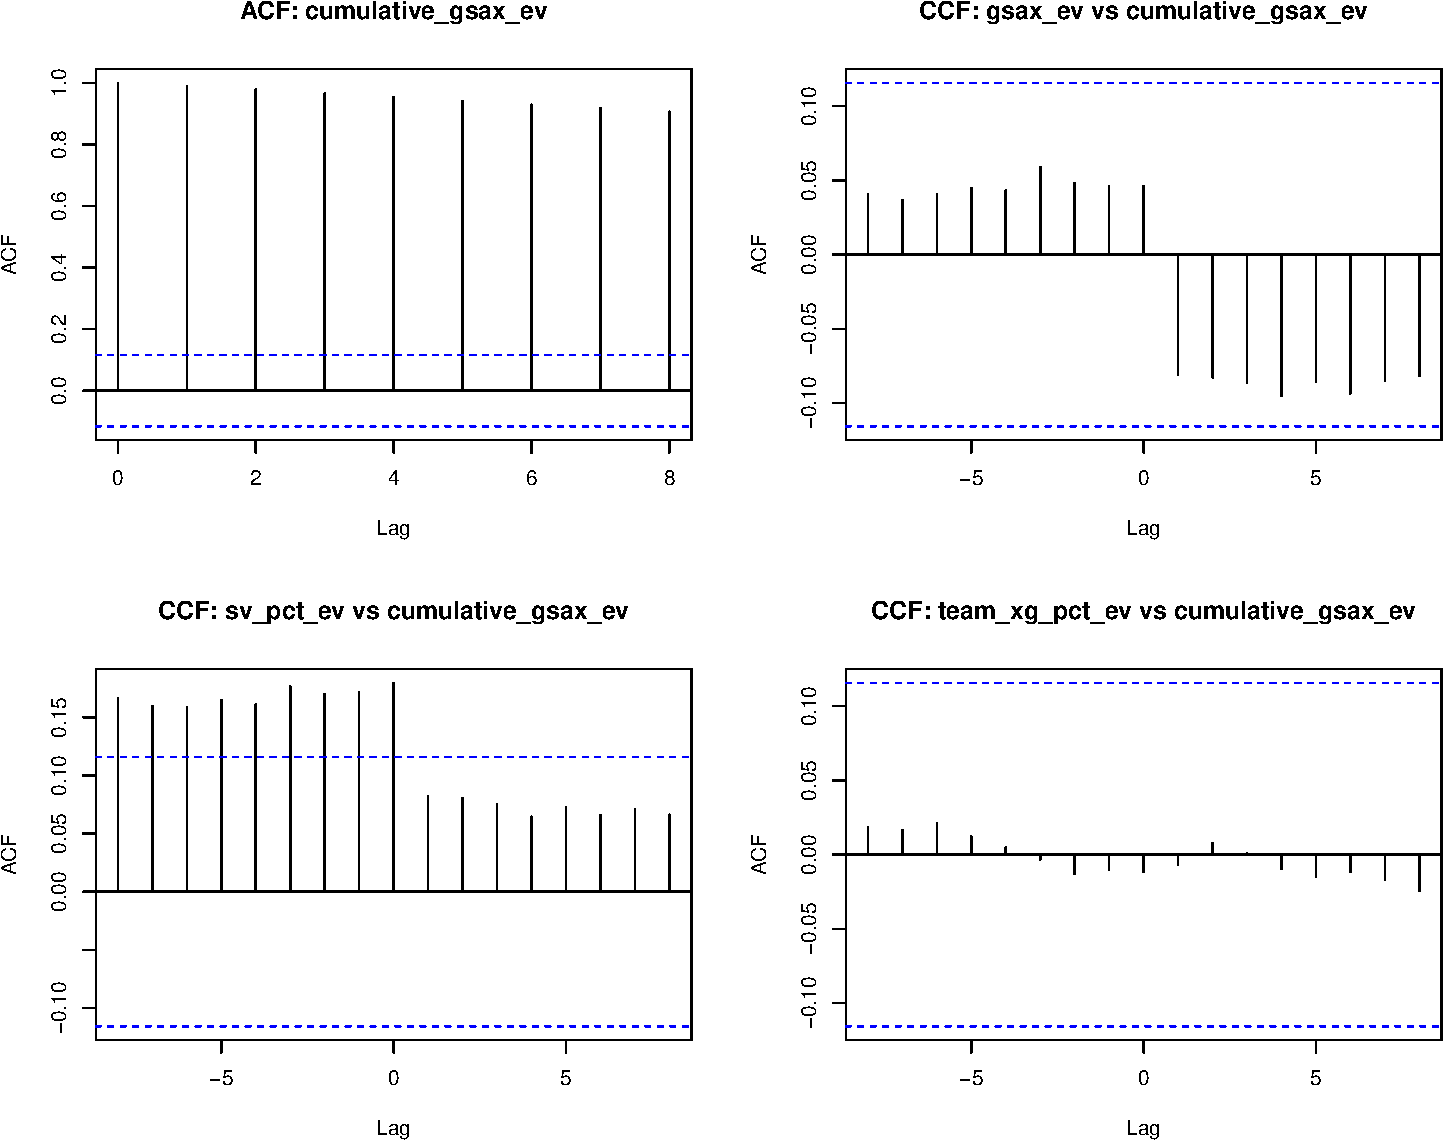
\includegraphics[width=\linewidth]{Homework4_files/figure-latex/unnamed-chunk-12-1} \end{center}

The ACF of \texttt{cumulative\_gsax\_ev} is extremely high at nearby lags, with lag-1 autocorrelation 0.989 and lag-4 autocorrelation 0.953. That is expected for a cumulative series and reinforces the idea that the mean structure is strongly time-dependent. Since our class regression approach has focused on modeling the mean directly with trend terms rather than adding lagged responses, I use this ACF mainly as evidence that a simple linear trend will not be enough.

For the CCFs, the noncontemporaneous lead-lag relation from \texttt{gsax\_ev} to \texttt{cumulative\_gsax\_ev} is weak, but among negative lags the largest spike occurs at lag -3 with correlation 0.059, so if I try a lagged GSAx predictor, \(G_{t-3}\) is the most defensible one. The CCF between \texttt{sv\_pct\_ev} and \texttt{cumulative\_gsax\_ev} is stronger, with a very large contemporaneous spike as expected, but among negative lags the largest spike occurs at lag -3 with correlation 0.176, so the natural lagged save-percentage predictor is \(S_{t-3}\). The CCF between \texttt{team\_xg\_pct\_ev} and \texttt{cumulative\_gsax\_ev} is extremely weak throughout, with the largest negative-lag spike only about 0.021 at lag -6, so I do not see enough evidence to keep \texttt{team\_xg\_pct\_ev} in the final candidate model set.

Let \(H_t\) denote \texttt{cumulative\_gsax\_ev}, let \(G_t\) denote \texttt{gsax\_ev}, and let \(S_t\) denote \texttt{sv\_pct\_ev}. Based on the non-linear shape in the response plot, the lack of seasonality in the periodogram, the strong persistence of the cumulative response, and the response-based CCFs, I compare the following six candidate models:

\[
\begin{aligned}
\text{Model I: } & H_t = \beta_0 + \beta_1 t + W_t, \\
\text{Model II: } & H_t = \beta_0 + \beta_1 t + \beta_2 \frac{t^2}{2!} + W_t, \\
\text{Model III: } & H_t = \beta_0 + \beta_1 t + \beta_2 \frac{t^2}{2!} + \beta_3 \frac{t^3}{3!} + W_t, \\
\text{Model IV: } & H_t = \beta_0 + \beta_1 t + \beta_2 \frac{t^2}{2!} + \beta_3 \frac{t^3}{3!} + \beta_4 S_{t-3} + W_t, \\
\text{Model V: } & H_t = \beta_0 + \beta_1 t + \beta_2 \frac{t^2}{2!} + \beta_3 \frac{t^3}{3!} + \beta_4 G_{t-3} + W_t, \\
\text{Model VI: } & H_t = \beta_0 + \beta_1 t + \beta_2 \frac{t^2}{2!} + \beta_3 \frac{t^3}{3!} + \beta_4 G_{t-3} + \beta_5 S_{t-3} + W_t.
\end{aligned}
\]

\begin{Shaded}
\begin{Highlighting}[]
\NormalTok{gsax\_forms }\OtherTok{\textless{}{-}} \FunctionTok{list}\NormalTok{(}
  \StringTok{\textquotesingle{}Model I\textquotesingle{}} \OtherTok{=}\NormalTok{ H }\SpecialCharTok{\textasciitilde{}}\NormalTok{ t,}
  \StringTok{\textquotesingle{}Model II\textquotesingle{}} \OtherTok{=}\NormalTok{ H }\SpecialCharTok{\textasciitilde{}}\NormalTok{ t }\SpecialCharTok{+}\NormalTok{ t2,}
  \StringTok{\textquotesingle{}Model III\textquotesingle{}} \OtherTok{=}\NormalTok{ H }\SpecialCharTok{\textasciitilde{}}\NormalTok{ t }\SpecialCharTok{+}\NormalTok{ t2 }\SpecialCharTok{+}\NormalTok{ t3,}
  \StringTok{\textquotesingle{}Model IV\textquotesingle{}} \OtherTok{=}\NormalTok{ H }\SpecialCharTok{\textasciitilde{}}\NormalTok{ t }\SpecialCharTok{+}\NormalTok{ t2 }\SpecialCharTok{+}\NormalTok{ t3 }\SpecialCharTok{+}\NormalTok{ SL3,}
  \StringTok{\textquotesingle{}Model V\textquotesingle{}} \OtherTok{=}\NormalTok{ H }\SpecialCharTok{\textasciitilde{}}\NormalTok{ t }\SpecialCharTok{+}\NormalTok{ t2 }\SpecialCharTok{+}\NormalTok{ t3 }\SpecialCharTok{+}\NormalTok{ GL3,}
  \StringTok{\textquotesingle{}Model VI\textquotesingle{}} \OtherTok{=}\NormalTok{ H }\SpecialCharTok{\textasciitilde{}}\NormalTok{ t }\SpecialCharTok{+}\NormalTok{ t2 }\SpecialCharTok{+}\NormalTok{ t3 }\SpecialCharTok{+}\NormalTok{ GL3 }\SpecialCharTok{+}\NormalTok{ SL3}
\NormalTok{)}

\NormalTok{models\_gsax }\OtherTok{\textless{}{-}} \FunctionTok{lapply}\NormalTok{(gsax\_forms, }\ControlFlowTok{function}\NormalTok{(form) stats}\SpecialCharTok{::}\FunctionTok{lm}\NormalTok{(form, }\AttributeTok{data =}\NormalTok{ gsax\_data))}
\NormalTok{gsax\_fit\_table }\OtherTok{\textless{}{-}} \FunctionTok{do.call}\NormalTok{(}
\NormalTok{  rbind,}
  \FunctionTok{lapply}\NormalTok{(}\FunctionTok{names}\NormalTok{(models\_gsax), }\ControlFlowTok{function}\NormalTok{(name) }\FunctionTok{cbind}\NormalTok{(}\AttributeTok{Model =}\NormalTok{ name, }\FunctionTok{fit\_table\_proj}\NormalTok{(models\_gsax[[name]])))}
\NormalTok{)}
\NormalTok{gsax\_fc\_table }\OtherTok{\textless{}{-}} \FunctionTok{do.call}\NormalTok{(}
\NormalTok{  rbind,}
  \FunctionTok{lapply}\NormalTok{(}\FunctionTok{names}\NormalTok{(gsax\_forms), }\ControlFlowTok{function}\NormalTok{(name) }\FunctionTok{cbind}\NormalTok{(}\AttributeTok{Model =}\NormalTok{ name, }\FunctionTok{fcst\_metrics\_proj}\NormalTok{(gsax\_data, gsax\_forms[[name]])))}
\NormalTok{)}
\FunctionTok{rownames}\NormalTok{(gsax\_fit\_table) }\OtherTok{\textless{}{-}} \ConstantTok{NULL}
\FunctionTok{rownames}\NormalTok{(gsax\_fc\_table) }\OtherTok{\textless{}{-}} \ConstantTok{NULL}
\NormalTok{gsax\_fit\_table}\SpecialCharTok{$}\NormalTok{Parameters }\OtherTok{\textless{}{-}} \FunctionTok{as.integer}\NormalTok{(gsax\_fit\_table}\SpecialCharTok{$}\NormalTok{Parameters)}

\NormalTok{gsax\_best }\OtherTok{\textless{}{-}}\NormalTok{ models\_gsax[[}\StringTok{\textquotesingle{}Model IV\textquotesingle{}}\NormalTok{]]}
\end{Highlighting}
\end{Shaded}

\begin{center}
\normalsize

\begin{tabular}{ccccccc}
\toprule
Model & \# Par & $R_a^2$ & $p_F$ & AIC & AICc & BIC\\
\midrule
Model I & 2 & 0.4066 & 0 & 7.0544 & 5.2168 & 7.0929\\
Model II & 3 & 0.5812 & 0 & 6.7094 & 4.8720 & 6.7608\\
Model III & 4 & 0.8170 & 0 & 5.8849 & 4.0478 & 5.9492\\
Model IV & 5 & 0.8204 & 0 & 5.8697 & 4.0329 & 5.9468\\
Model V & 5 & 0.8210 & 0 & 5.8664 & 4.0296 & 5.9435\\
\addlinespace
Model VI & 6 & 0.8206 & 0 & 5.8722 & 4.0357 & 5.9621\\
\bottomrule
\end{tabular}
\normalsize
\end{center}

\begin{center}
\normalsize

\begin{tabular}{cccccc}
\toprule
Model & ME & MPE & MSE & MAE & MAPE\\
\midrule
Model I & 18.5862 & -146.4454 & 417.2891 & 18.5862 & 146.4454\\
Model II & 30.4067 & -236.3151 & 1082.1976 & 30.4067 & 236.3151\\
Model III & -3.6883 & 39.0541 & 59.5635 & 5.7011 & 49.7332\\
Model IV & -2.9815 & 33.2417 & 49.6543 & 5.2292 & 45.1840\\
Model V & -3.3239 & 36.0647 & 53.2939 & 5.3759 & 46.9801\\
\addlinespace
Model VI & -3.0266 & 33.6143 & 49.9644 & 5.2379 & 45.3665\\
\bottomrule
\end{tabular}
\normalsize
\end{center}

\begin{Shaded}
\begin{Highlighting}[]
\CommentTok{\# Observed versus fitted plot for selected cumulative GSAx model.}
\NormalTok{astsa}\SpecialCharTok{::}\FunctionTok{tsplot}\NormalTok{(}
\NormalTok{  stats}\SpecialCharTok{::}\FunctionTok{ts}\NormalTok{(gsax\_data}\SpecialCharTok{$}\NormalTok{H, }\AttributeTok{start =} \FunctionTok{min}\NormalTok{(gsax\_data}\SpecialCharTok{$}\NormalTok{t), }\AttributeTok{frequency =} \DecValTok{1}\NormalTok{),}
  \AttributeTok{main =} \StringTok{\textquotesingle{}Observed vs Fitted cumulative\_gsax\_ev\textquotesingle{}}\NormalTok{,}
  \AttributeTok{xlab =} \StringTok{\textquotesingle{}Career Game Number (t)\textquotesingle{}}\NormalTok{,}
  \AttributeTok{ylab =} \StringTok{\textquotesingle{}Cumulative GSAx at EV (Goals)\textquotesingle{}}\NormalTok{,}
  \AttributeTok{col =} \StringTok{\textquotesingle{}black\textquotesingle{}}\NormalTok{,}
  \AttributeTok{lwd =} \DecValTok{2}
\NormalTok{)}
\FunctionTok{lines}\NormalTok{(}
\NormalTok{  stats}\SpecialCharTok{::}\FunctionTok{ts}\NormalTok{(stats}\SpecialCharTok{::}\FunctionTok{fitted}\NormalTok{(gsax\_best), }\AttributeTok{start =} \FunctionTok{min}\NormalTok{(gsax\_data}\SpecialCharTok{$}\NormalTok{t), }\AttributeTok{frequency =} \DecValTok{1}\NormalTok{),}
  \AttributeTok{col =} \StringTok{\textquotesingle{}darkgreen\textquotesingle{}}\NormalTok{,}
  \AttributeTok{lwd =} \DecValTok{2}
\NormalTok{)}
\NormalTok{graphics}\SpecialCharTok{::}\FunctionTok{legend}\NormalTok{(}\StringTok{\textquotesingle{}topleft\textquotesingle{}}\NormalTok{, }\AttributeTok{legend =} \FunctionTok{c}\NormalTok{(}\StringTok{\textquotesingle{}Observed\textquotesingle{}}\NormalTok{, }\StringTok{\textquotesingle{}Fitted\textquotesingle{}}\NormalTok{), }\AttributeTok{col =} \FunctionTok{c}\NormalTok{(}\StringTok{\textquotesingle{}black\textquotesingle{}}\NormalTok{, }\StringTok{\textquotesingle{}darkgreen\textquotesingle{}}\NormalTok{), }\AttributeTok{lty =} \DecValTok{1}\NormalTok{, }\AttributeTok{lwd =} \DecValTok{2}\NormalTok{, }\AttributeTok{bty =} \StringTok{\textquotesingle{}n\textquotesingle{}}\NormalTok{)}
\end{Highlighting}
\end{Shaded}

\begin{center}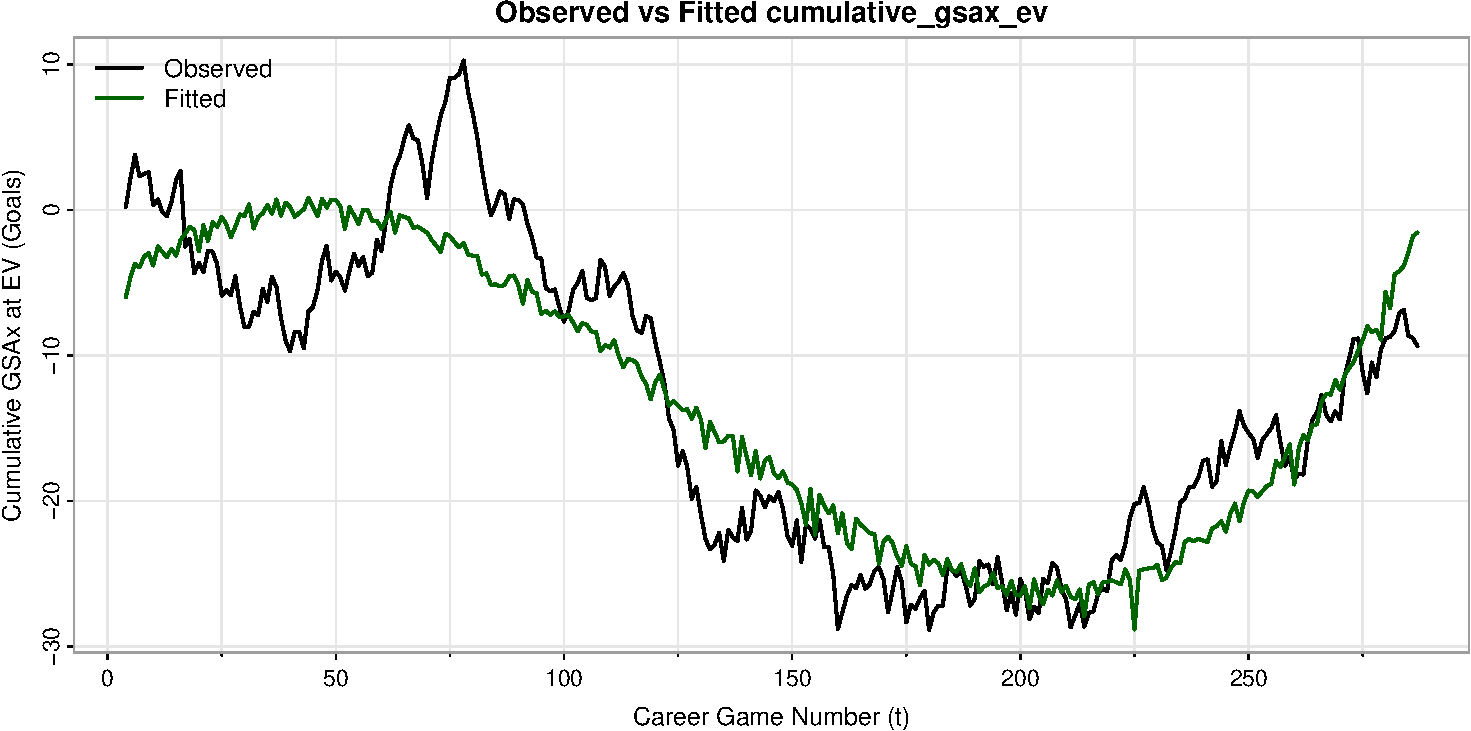
\includegraphics[width=\linewidth]{Homework4_files/figure-latex/unnamed-chunk-16-1} \end{center}

The comparison table shows that the linear and quadratic trend models are inadequate once the clear curvature of the series is taken seriously. Model III, the cubic trend model, is a major improvement over Models I and II. Among the lag-augmented models, the in-sample fit criteria slightly favor Model V, which adds the lag-3 GSAx term, but the forecast criteria favor Model IV, which adds the lag-3 save-percentage term. Model VI does not improve enough to justify keeping both lagged predictors together, since its added terms are not individually significant in the fuller model. Because the response-based CCF is stronger for \texttt{sv\_pct\_ev} than for \texttt{gsax\_ev}, and because Model IV gives the better holdout MSE and MAE, I select Model IV for \texttt{cumulative\_gsax\_ev}.

The fitted model is
\[
\widehat H_t
= -14.123338
+ 0.314215 t
- 0.008849 \frac{t^2}{2!}
+ 0.000071 \frac{t^3}{3!}
+ 8.67677 S_{t-3},
\]
where \(H_t\) is cumulative even-strength GSAx in goals and \(S_{t-3}\) is Blackwood's even-strength save percentage from three games earlier, measured in proportion form. Because Models IV-VI require the lagged terms, all six models are compared on the common aligned sample \(t=4,\ldots,287\), so \(n=284\). The lag-3 \texttt{sv\_pct\_ev} coefficient is statistically significant with \(p = 0.0128\), which is consistent with the strongest noncontemporaneous CCF relation among the candidate predictors. The coefficient of determination is \(R^2 = 0.8229\), so the model explains about 82.29\% of the variation in \texttt{cumulative\_gsax\_ev}. The residual standard error is 4.4982 cumulative-GSAx units, which means on average the fitted cumulative even-strength GSAx differs from the observed cumulative even-strength GSAx by about 4.4982 goals. Because \texttt{cumulative\_gsax\_ev} can be negative or near zero, the percent-based holdout errors MPE and MAPE are less stable here than MSE and MAE, so I rely more on the latter two when discussing forecast performance.

In summary, the even-strength evidence does not suggest any meaningful seasonal cycle in cumulative GSAx, so seasonal terms are unnecessary. The time-series plot supports a cubic trend, the ACF confirms that the cumulative response is highly persistent, and the response-based CCFs suggest that lagged save percentage is the most relevant noncontemporaneous predictor among the candidate variables, while \texttt{team\_xg\_pct\_ev} does not show much direct signal against \texttt{cumulative\_gsax\_ev} in this one-goalie setting. So at this stage, the results do not give strong evidence that the measured team-context variable I used is driving cumulative GSAx, but they do suggest that recent goalie-level performance still matters, which means the broader ``GSAx is fully independent of circumstance'' claim remains unsettled rather than confirmed. One limitation is that these exploratory diagnostics were examined on the full dataset before the train-holdout split was used for forecast evaluation, so there is some information leakage in the model-building stage. Also, \texttt{team\_xg\_pct\_ev} is only one public context measure, and the xG model itself still misses information such as detailed pre-shot passing structure. With those limitations noted, Model IV is my final choice for now because it is the best current working model for this stage of the project, not the permanent final conclusion on the research question.

\end{document}
